\documentclass[twoside]{book}

% Packages required by doxygen
\usepackage{fixltx2e}
\usepackage{calc}
\usepackage{doxygen}
\usepackage[export]{adjustbox} % also loads graphicx
\usepackage{graphicx}
\usepackage[utf8]{inputenc}
\usepackage{makeidx}
\usepackage{multicol}
\usepackage{multirow}
\PassOptionsToPackage{warn}{textcomp}
\usepackage{textcomp}
\usepackage[nointegrals]{wasysym}
\usepackage[table]{xcolor}

% Font selection
\usepackage[T1]{fontenc}
\usepackage[scaled=.90]{helvet}
\usepackage{courier}
\usepackage{amssymb}
\usepackage{sectsty}
\renewcommand{\familydefault}{\sfdefault}
\allsectionsfont{%
  \fontseries{bc}\selectfont%
  \color{darkgray}%
}
\renewcommand{\DoxyLabelFont}{%
  \fontseries{bc}\selectfont%
  \color{darkgray}%
}
\newcommand{\+}{\discretionary{\mbox{\scriptsize$\hookleftarrow$}}{}{}}

% Page & text layout
\usepackage{geometry}
\geometry{%
  a4paper,%
  top=2.5cm,%
  bottom=2.5cm,%
  left=2.5cm,%
  right=2.5cm%
}
\tolerance=750
\hfuzz=15pt
\hbadness=750
\setlength{\emergencystretch}{15pt}
\setlength{\parindent}{0cm}
\setlength{\parskip}{3ex plus 2ex minus 2ex}
\makeatletter
\renewcommand{\paragraph}{%
  \@startsection{paragraph}{4}{0ex}{-1.0ex}{1.0ex}{%
    \normalfont\normalsize\bfseries\SS@parafont%
  }%
}
\renewcommand{\subparagraph}{%
  \@startsection{subparagraph}{5}{0ex}{-1.0ex}{1.0ex}{%
    \normalfont\normalsize\bfseries\SS@subparafont%
  }%
}
\makeatother

% Headers & footers
\usepackage{fancyhdr}
\pagestyle{fancyplain}
\fancyhead[LE]{\fancyplain{}{\bfseries\thepage}}
\fancyhead[CE]{\fancyplain{}{}}
\fancyhead[RE]{\fancyplain{}{\bfseries\leftmark}}
\fancyhead[LO]{\fancyplain{}{\bfseries\rightmark}}
\fancyhead[CO]{\fancyplain{}{}}
\fancyhead[RO]{\fancyplain{}{\bfseries\thepage}}
\fancyfoot[LE]{\fancyplain{}{}}
\fancyfoot[CE]{\fancyplain{}{}}
\fancyfoot[RE]{\fancyplain{}{\bfseries\scriptsize Generated by Doxygen }}
\fancyfoot[LO]{\fancyplain{}{\bfseries\scriptsize Generated by Doxygen }}
\fancyfoot[CO]{\fancyplain{}{}}
\fancyfoot[RO]{\fancyplain{}{}}
\renewcommand{\footrulewidth}{0.4pt}
\renewcommand{\chaptermark}[1]{%
  \markboth{#1}{}%
}
\renewcommand{\sectionmark}[1]{%
  \markright{\thesection\ #1}%
}

% Indices & bibliography
\usepackage{natbib}
\usepackage[titles]{tocloft}
\setcounter{tocdepth}{3}
\setcounter{secnumdepth}{5}
\makeindex

% Hyperlinks (required, but should be loaded last)
\usepackage{ifpdf}
\ifpdf
  \usepackage[pdftex,pagebackref=true]{hyperref}
\else
  \usepackage[ps2pdf,pagebackref=true]{hyperref}
\fi
\hypersetup{%
  colorlinks=true,%
  linkcolor=blue,%
  citecolor=blue,%
  unicode%
}

% Custom commands
\newcommand{\clearemptydoublepage}{%
  \newpage{\pagestyle{empty}\cleardoublepage}%
}

\usepackage{caption}
\captionsetup{labelsep=space,justification=centering,font={bf},singlelinecheck=off,skip=4pt,position=top}

%===== C O N T E N T S =====

\begin{document}

% Titlepage & ToC
\hypersetup{pageanchor=false,
             bookmarksnumbered=true,
             pdfencoding=unicode
            }
\pagenumbering{alph}
\begin{titlepage}
\vspace*{7cm}
\begin{center}%
{\Large Dataset Labelling Tool }\\
\vspace*{1cm}
{\large Generated by Doxygen 1.8.13}\\
\end{center}
\end{titlepage}
\clearemptydoublepage
\pagenumbering{roman}
\tableofcontents
\clearemptydoublepage
\pagenumbering{arabic}
\hypersetup{pageanchor=true}

%--- Begin generated contents ---
\chapter{Hierarchical Index}
\section{Class Hierarchy}
This inheritance list is sorted roughly, but not completely, alphabetically\+:\begin{DoxyCompactList}
\item \contentsline{section}{Annotation\+Controller}{\pageref{classAnnotationController}}{}
\item \contentsline{section}{Annotation\+Model}{\pageref{classAnnotationModel}}{}
\item \contentsline{section}{Class\+Controller}{\pageref{classClassController}}{}
\item \contentsline{section}{Class\+Model}{\pageref{classClassModel}}{}
\item exception\begin{DoxyCompactList}
\item \contentsline{section}{Array\+Empty\+Error}{\pageref{classArrayEmptyError}}{}
\item \contentsline{section}{Class\+Not\+Found\+Error}{\pageref{classClassNotFoundError}}{}
\item \contentsline{section}{Class\+Not\+Selected\+Error}{\pageref{classClassNotSelectedError}}{}
\item \contentsline{section}{Drawing\+Incomplete}{\pageref{classDrawingIncomplete}}{}
\item \contentsline{section}{File\+Not\+Found\+Error}{\pageref{classFileNotFoundError}}{}
\item \contentsline{section}{Folder\+Not\+Found\+Error}{\pageref{classFolderNotFoundError}}{}
\item \contentsline{section}{Image\+Not\+Annotated\+Yet}{\pageref{classImageNotAnnotatedYet}}{}
\item \contentsline{section}{Index\+Out\+Of\+Bounds\+Error}{\pageref{classIndexOutOfBoundsError}}{}
\item \contentsline{section}{Operation\+Canceled}{\pageref{classOperationCanceled}}{}
\item \contentsline{section}{Value\+Not\+Found\+Error}{\pageref{classValueNotFoundError}}{}
\end{DoxyCompactList}
\item \contentsline{section}{Image\+Controller}{\pageref{classImageController}}{}
\item \contentsline{section}{Image\+Model}{\pageref{classImageModel}}{}
\item \contentsline{section}{Linked\+List$<$ T $>$}{\pageref{classLinkedList}}{}
\item \contentsline{section}{Linked\+List$<$ Q\+Pair$<$ Q\+String, Q\+Vector$<$ Q\+PointF $>$ $>$ $>$}{\pageref{classLinkedList}}{}
\item \contentsline{section}{Linked\+List$<$ Q\+String $>$}{\pageref{classLinkedList}}{}
\item \contentsline{section}{Main\+Controller}{\pageref{classMainController}}{}
\item \contentsline{section}{Linked\+List$<$ T $>$\+:\+:Node}{\pageref{structLinkedList_1_1Node}}{}
\item Q\+Graphics\+View\begin{DoxyCompactList}
\item \contentsline{section}{Graphics\+View}{\pageref{classGraphicsView}}{}
\end{DoxyCompactList}
\item Q\+Main\+Window\begin{DoxyCompactList}
\item \contentsline{section}{Main\+View}{\pageref{classMainView}}{}
\end{DoxyCompactList}
\end{DoxyCompactList}

\chapter{Class Index}
\section{Class List}
Here are the classes, structs, unions and interfaces with brief descriptions\+:\begin{DoxyCompactList}
\item\contentsline{section}{\hyperlink{classAnnotationController}{Annotation\+Controller} }{\pageref{classAnnotationController}}{}
\item\contentsline{section}{\hyperlink{classAnnotationModel}{Annotation\+Model} }{\pageref{classAnnotationModel}}{}
\item\contentsline{section}{\hyperlink{classArrayEmptyError}{Array\+Empty\+Error} }{\pageref{classArrayEmptyError}}{}
\item\contentsline{section}{\hyperlink{classClassController}{Class\+Controller} }{\pageref{classClassController}}{}
\item\contentsline{section}{\hyperlink{classClassModel}{Class\+Model} }{\pageref{classClassModel}}{}
\item\contentsline{section}{\hyperlink{classFileNotFoundError}{File\+Not\+Found\+Error} }{\pageref{classFileNotFoundError}}{}
\item\contentsline{section}{\hyperlink{classFolderNotFoundError}{Folder\+Not\+Found\+Error} }{\pageref{classFolderNotFoundError}}{}
\item\contentsline{section}{\hyperlink{classImageController}{Image\+Controller} }{\pageref{classImageController}}{}
\item\contentsline{section}{\hyperlink{classImageModel}{Image\+Model} }{\pageref{classImageModel}}{}
\item\contentsline{section}{\hyperlink{classImageNotAnnotatedYet}{Image\+Not\+Annotated\+Yet} }{\pageref{classImageNotAnnotatedYet}}{}
\item\contentsline{section}{\hyperlink{classIndexOutOfBoundsError}{Index\+Out\+Of\+Bounds\+Error} }{\pageref{classIndexOutOfBoundsError}}{}
\item\contentsline{section}{\hyperlink{classLinkedList}{Linked\+List$<$ T $>$} }{\pageref{classLinkedList}}{}
\item\contentsline{section}{\hyperlink{classMainController}{Main\+Controller} }{\pageref{classMainController}}{}
\item\contentsline{section}{\hyperlink{classMainView}{Main\+View} }{\pageref{classMainView}}{}
\item\contentsline{section}{\hyperlink{structLinkedList_1_1Node}{Linked\+List$<$ T $>$\+::\+Node} }{\pageref{structLinkedList_1_1Node}}{}
\item\contentsline{section}{\hyperlink{classOperationCanceled}{Operation\+Canceled} }{\pageref{classOperationCanceled}}{}
\item\contentsline{section}{\hyperlink{classValueNotFoundError}{Value\+Not\+Found\+Error} }{\pageref{classValueNotFoundError}}{}
\end{DoxyCompactList}

\chapter{Class Documentation}
\hypertarget{classAnnotationController}{}\section{Annotation\+Controller Class Reference}
\label{classAnnotationController}\index{Annotation\+Controller@{Annotation\+Controller}}


{\ttfamily \#include $<$Annotation\+Controller.\+h$>$}



Collaboration diagram for Annotation\+Controller\+:
\nopagebreak
\begin{figure}[H]
\begin{center}
\leavevmode
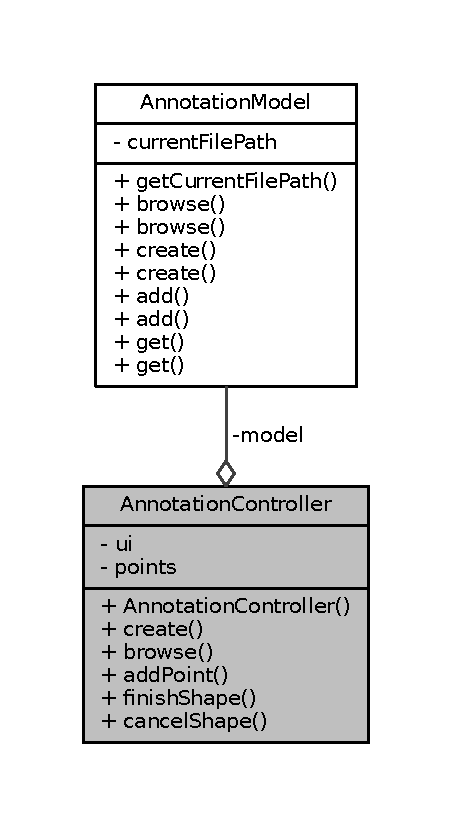
\includegraphics[width=217pt]{classAnnotationController__coll__graph}
\end{center}
\end{figure}
\subsection*{Public Member Functions}
\begin{DoxyCompactItemize}
\item 
\hyperlink{classAnnotationController_a28cad1eb39c829d54093a965f59cdb2e}{Annotation\+Controller} (const Ui\+\_\+\+Main\+View \&, const \hyperlink{classAnnotationModel}{Annotation\+Model} \&)
\begin{DoxyCompactList}\small\item\em Constructs an Annotation Controller, which handles logic related to the annotation files. \end{DoxyCompactList}\item 
\mbox{\Hypertarget{classAnnotationController_a490f659b6a1b6f4740925871689f747b}\label{classAnnotationController_a490f659b6a1b6f4740925871689f747b}} 
void {\bfseries create} ()
\item 
\mbox{\Hypertarget{classAnnotationController_aa79d79caa93863d2676900cece4cc994}\label{classAnnotationController_aa79d79caa93863d2676900cece4cc994}} 
void \hyperlink{classAnnotationController_aa79d79caa93863d2676900cece4cc994}{browse} ()
\begin{DoxyCompactList}\small\item\em Creates an annotation file and updates label in the UI accordingly. \end{DoxyCompactList}\item 
\mbox{\Hypertarget{classAnnotationController_a03b1715610f84b203e7a5ded7046dcd2}\label{classAnnotationController_a03b1715610f84b203e7a5ded7046dcd2}} 
void {\bfseries add\+Point} (Point)
\item 
\mbox{\Hypertarget{classAnnotationController_a295ef2113a2ef2201e736240e7a1078a}\label{classAnnotationController_a295ef2113a2ef2201e736240e7a1078a}} 
void {\bfseries finish\+Shape} ()
\item 
\mbox{\Hypertarget{classAnnotationController_aff95935a2215c4a52cbeb2674317d17d}\label{classAnnotationController_aff95935a2215c4a52cbeb2674317d17d}} 
void {\bfseries cancel\+Shape} ()
\end{DoxyCompactItemize}
\subsection*{Private Attributes}
\begin{DoxyCompactItemize}
\item 
\mbox{\Hypertarget{classAnnotationController_ad6db968693628859a69bab0667006dc1}\label{classAnnotationController_ad6db968693628859a69bab0667006dc1}} 
Ui\+\_\+\+Main\+View {\bfseries ui}
\item 
\mbox{\Hypertarget{classAnnotationController_ac9fc70313798905bf9fca275edfda08e}\label{classAnnotationController_ac9fc70313798905bf9fca275edfda08e}} 
\hyperlink{classAnnotationModel}{Annotation\+Model} {\bfseries model}
\item 
\mbox{\Hypertarget{classAnnotationController_aa4d49b736dedbd57d47c74ab3cef65cc}\label{classAnnotationController_aa4d49b736dedbd57d47c74ab3cef65cc}} 
std\+::vector$<$ Point $>$ {\bfseries points}
\end{DoxyCompactItemize}


\subsection{Detailed Description}
Sub-\/controller which gets delegated tasks related to annotation files. Communicates directly with the \hyperlink{classAnnotationModel}{Annotation\+Model}. 

\subsection{Constructor \& Destructor Documentation}
\mbox{\Hypertarget{classAnnotationController_a28cad1eb39c829d54093a965f59cdb2e}\label{classAnnotationController_a28cad1eb39c829d54093a965f59cdb2e}} 
\index{Annotation\+Controller@{Annotation\+Controller}!Annotation\+Controller@{Annotation\+Controller}}
\index{Annotation\+Controller@{Annotation\+Controller}!Annotation\+Controller@{Annotation\+Controller}}
\subsubsection{\texorpdfstring{Annotation\+Controller()}{AnnotationController()}}
{\footnotesize\ttfamily Annotation\+Controller\+::\+Annotation\+Controller (\begin{DoxyParamCaption}\item[{const Ui\+\_\+\+Main\+View \&}]{ui,  }\item[{const \hyperlink{classAnnotationModel}{Annotation\+Model} \&}]{model }\end{DoxyParamCaption})}



Constructs an Annotation Controller, which handles logic related to the annotation files. 


\begin{DoxyParams}{Parameters}
{\em ui} & The Ui\+\_\+\+Main\+View reference, which is used to update the G\+UI. \\
\hline
{\em model} & The \hyperlink{classAnnotationModel}{Annotation\+Model} that the \hyperlink{classAnnotationController}{Annotation\+Controller} accesses. \\
\hline
\end{DoxyParams}


The documentation for this class was generated from the following files\+:\begin{DoxyCompactItemize}
\item 
include/Annotation\+Controller.\+h\item 
src/Annotation\+Controller.\+cpp\end{DoxyCompactItemize}

\hypertarget{classAnnotationModel}{}\section{Annotation\+Model Class Reference}
\label{classAnnotationModel}\index{Annotation\+Model@{Annotation\+Model}}


{\ttfamily \#include $<$Annotation\+Model.\+h$>$}



Collaboration diagram for Annotation\+Model\+:
\nopagebreak
\begin{figure}[H]
\begin{center}
\leavevmode
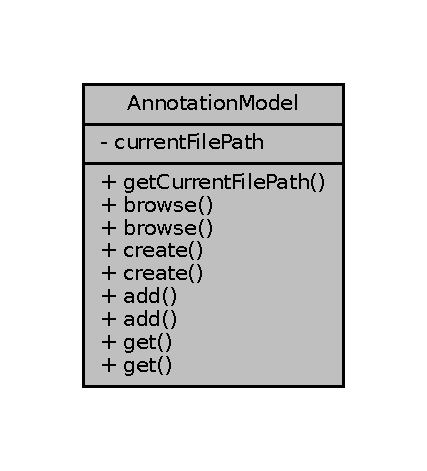
\includegraphics[width=205pt]{classAnnotationModel__coll__graph}
\end{center}
\end{figure}
\subsection*{Public Member Functions}
\begin{DoxyCompactItemize}
\item 
Q\+String \hyperlink{classAnnotationModel_a704170b9d4cc9e6b62e0bc22d17f6e17}{get\+Current\+File\+Path} ()
\begin{DoxyCompactList}\small\item\em Returns path of currently active annotation file. \end{DoxyCompactList}\item 
void \hyperlink{classAnnotationModel_aa43f69c5431ede4dc744ae9b61b49f6c}{browse} ()
\begin{DoxyCompactList}\small\item\em Prompts user to navigate to a annotation file on the system. \end{DoxyCompactList}\item 
void \hyperlink{classAnnotationModel_a54f9ffa4151a1bdcaa1d5ab3dee87679}{browse} (const Q\+String \&)
\begin{DoxyCompactList}\small\item\em Provides a way to enter path to annotation file as a parameter (Q\+String). \end{DoxyCompactList}\item 
void \hyperlink{classAnnotationModel_ac4c6850c8d0f704c3bf5bef486992690}{create} ()
\begin{DoxyCompactList}\small\item\em Prompts the user for a annotation file name. Creates a file using this name and path. \end{DoxyCompactList}\item 
void \hyperlink{classAnnotationModel_ac5062c8663670a312132929f16e4be64}{create} (const Q\+String \&)
\begin{DoxyCompactList}\small\item\em Provides a way to create annotation file by providing file path as a parameter (Q\+String) \end{DoxyCompactList}\item 
\mbox{\Hypertarget{classAnnotationModel_a4b6bbcae3cae275254085c857609413e}\label{classAnnotationModel_a4b6bbcae3cae275254085c857609413e}} 
void {\bfseries add} (const Q\+String \&json\+File\+Path, const Q\+String \&image\+File\+Path, const Q\+String \&class\+Name, \hyperlink{classLinkedList}{Linked\+List}$<$ Q\+Pair$<$ int, int $>$$>$ \&coordinates)
\item 
\mbox{\Hypertarget{classAnnotationModel_a58af7fa7e9af062292bcb0ce531f95a6}\label{classAnnotationModel_a58af7fa7e9af062292bcb0ce531f95a6}} 
void {\bfseries add} (const Q\+String \&image\+File\+Path, const Q\+String \&class\+Name, \hyperlink{classLinkedList}{Linked\+List}$<$ Q\+Pair$<$ int, int $>$$>$ \&coordinates)
\item 
Q\+Map$<$ Q\+String, \hyperlink{classLinkedList}{Shape} $>$ \hyperlink{classAnnotationModel_a242d12f3043434463c061b4a38d27c90}{get} (const Q\+String \&)
\begin{DoxyCompactList}\small\item\em Provides a way to obtain annotations for a given image from currently loaded annotation file. \end{DoxyCompactList}\item 
Q\+Map$<$ Q\+String, \hyperlink{classLinkedList}{Shape} $>$ \hyperlink{classAnnotationModel_afed52e5d48da396919f02ed88c94921a}{get} (const Q\+String \&, const Q\+String \&)
\begin{DoxyCompactList}\small\item\em Provides a way to obtain annotations for a given image from a specified annotation file. \end{DoxyCompactList}\end{DoxyCompactItemize}
\subsection*{Private Attributes}
\begin{DoxyCompactItemize}
\item 
\mbox{\Hypertarget{classAnnotationModel_a204571a62dfdc60a405528ddc1db2a61}\label{classAnnotationModel_a204571a62dfdc60a405528ddc1db2a61}} 
Q\+String {\bfseries current\+File\+Path}
\end{DoxyCompactItemize}


\subsection{Detailed Description}
Model, which is responsible for accessing annotation data. 

\subsection{Member Function Documentation}
\mbox{\Hypertarget{classAnnotationModel_aa43f69c5431ede4dc744ae9b61b49f6c}\label{classAnnotationModel_aa43f69c5431ede4dc744ae9b61b49f6c}} 
\index{Annotation\+Model@{Annotation\+Model}!browse@{browse}}
\index{browse@{browse}!Annotation\+Model@{Annotation\+Model}}
\subsubsection{\texorpdfstring{browse()}{browse()}\hspace{0.1cm}{\footnotesize\ttfamily [1/2]}}
{\footnotesize\ttfamily void Annotation\+Model\+::browse (\begin{DoxyParamCaption}{ }\end{DoxyParamCaption})}



Prompts user to navigate to a annotation file on the system. 

If entered path is empty, or file could not be oppened, std\+::invalid\+\_\+argument exception is thrown. If operation is canceled custom \hyperlink{classOperationCanceled}{Operation\+Canceled} exception is thrown. Location of opened file is saved to a private current\+File\+Path attribute in this class. \mbox{\Hypertarget{classAnnotationModel_a54f9ffa4151a1bdcaa1d5ab3dee87679}\label{classAnnotationModel_a54f9ffa4151a1bdcaa1d5ab3dee87679}} 
\index{Annotation\+Model@{Annotation\+Model}!browse@{browse}}
\index{browse@{browse}!Annotation\+Model@{Annotation\+Model}}
\subsubsection{\texorpdfstring{browse()}{browse()}\hspace{0.1cm}{\footnotesize\ttfamily [2/2]}}
{\footnotesize\ttfamily void Annotation\+Model\+::browse (\begin{DoxyParamCaption}\item[{const Q\+String \&}]{file\+Path }\end{DoxyParamCaption})}



Provides a way to enter path to annotation file as a parameter (Q\+String). 

If entered path is empty, or file could not be oppened, std\+::invalid\+\_\+argument exception is thrown. Location of opened file is saved to a private current\+File\+Path attribute in this class.


\begin{DoxyParams}{Parameters}
{\em file\+Path} & Q\+String path for a annotation file you want to create. \\
\hline
\end{DoxyParams}
\mbox{\Hypertarget{classAnnotationModel_ac4c6850c8d0f704c3bf5bef486992690}\label{classAnnotationModel_ac4c6850c8d0f704c3bf5bef486992690}} 
\index{Annotation\+Model@{Annotation\+Model}!create@{create}}
\index{create@{create}!Annotation\+Model@{Annotation\+Model}}
\subsubsection{\texorpdfstring{create()}{create()}\hspace{0.1cm}{\footnotesize\ttfamily [1/2]}}
{\footnotesize\ttfamily void Annotation\+Model\+::create (\begin{DoxyParamCaption}{ }\end{DoxyParamCaption})}



Prompts the user for a annotation file name. Creates a file using this name and path. 

If file\+Path is empty, or file could not be created at wanted location std\+::invalid argument exception is thrown. If operation is canceled custom \hyperlink{classOperationCanceled}{Operation\+Canceled} exception is thrown. Location of opened file is saved to a private current\+File\+Path attribute in this class. \mbox{\Hypertarget{classAnnotationModel_ac5062c8663670a312132929f16e4be64}\label{classAnnotationModel_ac5062c8663670a312132929f16e4be64}} 
\index{Annotation\+Model@{Annotation\+Model}!create@{create}}
\index{create@{create}!Annotation\+Model@{Annotation\+Model}}
\subsubsection{\texorpdfstring{create()}{create()}\hspace{0.1cm}{\footnotesize\ttfamily [2/2]}}
{\footnotesize\ttfamily void Annotation\+Model\+::create (\begin{DoxyParamCaption}\item[{const Q\+String \&}]{file\+Path }\end{DoxyParamCaption})}



Provides a way to create annotation file by providing file path as a parameter (Q\+String) 

If file\+Path is empty, or file could not be created at wanted location std\+::invalid argument exception is thrown. Location of opened file is saved to a private current\+File\+Path attribute in this class.


\begin{DoxyParams}{Parameters}
{\em file\+Path} & Q\+String path for a annotation file you want to create. \\
\hline
\end{DoxyParams}
\mbox{\Hypertarget{classAnnotationModel_a242d12f3043434463c061b4a38d27c90}\label{classAnnotationModel_a242d12f3043434463c061b4a38d27c90}} 
\index{Annotation\+Model@{Annotation\+Model}!get@{get}}
\index{get@{get}!Annotation\+Model@{Annotation\+Model}}
\subsubsection{\texorpdfstring{get()}{get()}\hspace{0.1cm}{\footnotesize\ttfamily [1/2]}}
{\footnotesize\ttfamily Q\+Map$<$ Q\+String, \hyperlink{classLinkedList}{Linked\+List}$<$ Q\+Pair$<$ int, int $>$ $>$ $>$ Annotation\+Model\+::get (\begin{DoxyParamCaption}\item[{const Q\+String \&}]{image\+Name }\end{DoxyParamCaption})}



Provides a way to obtain annotations for a given image from currently loaded annotation file. 

Function searches for all annotations which are made for image name provided in a parameter. If provided image is not annotated in currenlly loaded annotation file, custom \hyperlink{classImageNotAnnotatedYet}{Image\+Not\+Annotated\+Yet} exception is thrown.


\begin{DoxyParams}{Parameters}
{\em image\+Name} & Q\+String name of the image user wants to obtain. \\
\hline
\end{DoxyParams}
\begin{DoxyReturn}{Returns}
Q\+Map of annotations, key being class name and value being \hyperlink{classLinkedList}{Linked\+List} of Q\+Pair. 
\end{DoxyReturn}
\mbox{\Hypertarget{classAnnotationModel_afed52e5d48da396919f02ed88c94921a}\label{classAnnotationModel_afed52e5d48da396919f02ed88c94921a}} 
\index{Annotation\+Model@{Annotation\+Model}!get@{get}}
\index{get@{get}!Annotation\+Model@{Annotation\+Model}}
\subsubsection{\texorpdfstring{get()}{get()}\hspace{0.1cm}{\footnotesize\ttfamily [2/2]}}
{\footnotesize\ttfamily Q\+Map$<$ Q\+String, \hyperlink{classLinkedList}{Linked\+List}$<$ Q\+Pair$<$ int, int $>$ $>$ $>$ Annotation\+Model\+::get (\begin{DoxyParamCaption}\item[{const Q\+String \&}]{image\+Name,  }\item[{const Q\+String \&}]{file\+Path }\end{DoxyParamCaption})}



Provides a way to obtain annotations for a given image from a specified annotation file. 

Function searches for all annotations which are made for image name provided in a parameter. If provided image is not annotated in currenlly loaded annotation file, custom \hyperlink{classImageNotAnnotatedYet}{Image\+Not\+Annotated\+Yet} exception is thrown.


\begin{DoxyParams}{Parameters}
{\em image\+Name} & Q\+String name of the image user wants to obtain. \\
\hline
{\em file\+Path} & Q\+String path to annotation file where annotation for the image should be looked for. \\
\hline
\end{DoxyParams}
\begin{DoxyReturn}{Returns}
Q\+Map of annotations, key being class name and value being \hyperlink{classLinkedList}{Linked\+List} of Q\+Pair. 
\end{DoxyReturn}
\mbox{\Hypertarget{classAnnotationModel_a704170b9d4cc9e6b62e0bc22d17f6e17}\label{classAnnotationModel_a704170b9d4cc9e6b62e0bc22d17f6e17}} 
\index{Annotation\+Model@{Annotation\+Model}!get\+Current\+File\+Path@{get\+Current\+File\+Path}}
\index{get\+Current\+File\+Path@{get\+Current\+File\+Path}!Annotation\+Model@{Annotation\+Model}}
\subsubsection{\texorpdfstring{get\+Current\+File\+Path()}{getCurrentFilePath()}}
{\footnotesize\ttfamily Q\+String Annotation\+Model\+::get\+Current\+File\+Path (\begin{DoxyParamCaption}{ }\end{DoxyParamCaption})}



Returns path of currently active annotation file. 

\begin{DoxyReturn}{Returns}
Path to a annotation file. 
\end{DoxyReturn}


The documentation for this class was generated from the following files\+:\begin{DoxyCompactItemize}
\item 
include/Annotation\+Model.\+h\item 
src/Annotation\+Model.\+cpp\end{DoxyCompactItemize}

\hypertarget{classArrayEmptyError}{}\section{Array\+Empty\+Error Class Reference}
\label{classArrayEmptyError}\index{Array\+Empty\+Error@{Array\+Empty\+Error}}


{\ttfamily \#include $<$exceptions.\+h$>$}



Inheritance diagram for Array\+Empty\+Error\+:\nopagebreak
\begin{figure}[H]
\begin{center}
\leavevmode
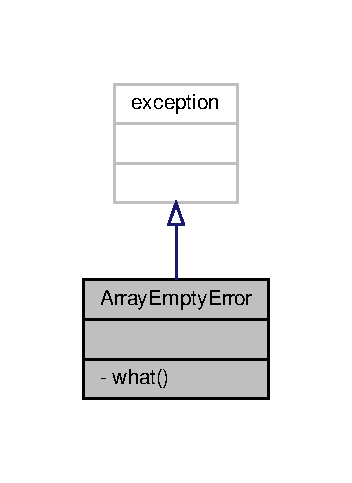
\includegraphics[width=169pt]{classArrayEmptyError__inherit__graph}
\end{center}
\end{figure}


Collaboration diagram for Array\+Empty\+Error\+:\nopagebreak
\begin{figure}[H]
\begin{center}
\leavevmode
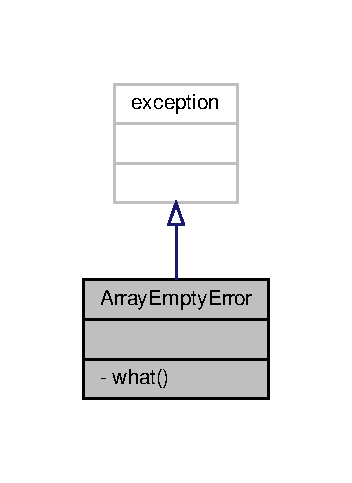
\includegraphics[width=169pt]{classArrayEmptyError__coll__graph}
\end{center}
\end{figure}
\subsection*{Private Member Functions}
\begin{DoxyCompactItemize}
\item 
\mbox{\Hypertarget{classArrayEmptyError_a5a24151f18d18d9c04df7925a7494d77}\label{classArrayEmptyError_a5a24151f18d18d9c04df7925a7494d77}} 
const char $\ast$ {\bfseries what} () const  throw ()
\end{DoxyCompactItemize}


\subsection{Detailed Description}
Custom exception subclass, which signifies an empty array. 

The documentation for this class was generated from the following file\+:\begin{DoxyCompactItemize}
\item 
include/exceptions.\+h\end{DoxyCompactItemize}

\hypertarget{classClassController}{}\section{Class\+Controller Class Reference}
\label{classClassController}\index{Class\+Controller@{Class\+Controller}}


{\ttfamily \#include $<$Class\+Controller.\+h$>$}



Collaboration diagram for Class\+Controller\+:
\nopagebreak
\begin{figure}[H]
\begin{center}
\leavevmode
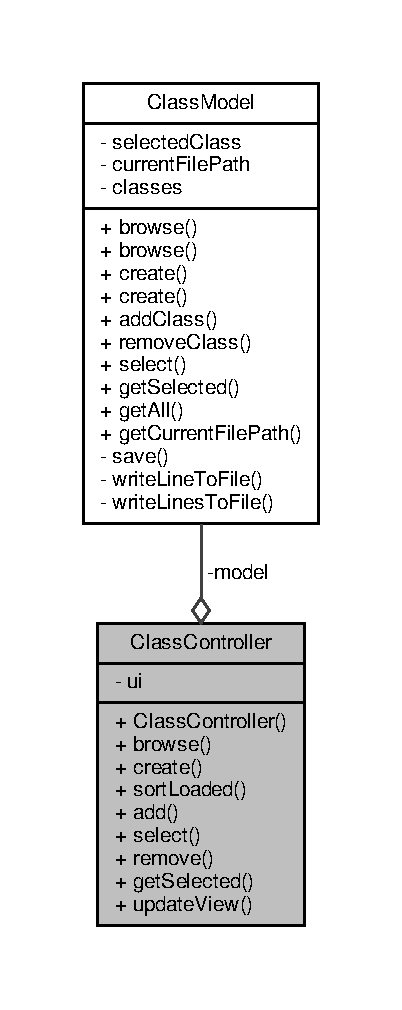
\includegraphics[height=550pt]{classClassController__coll__graph}
\end{center}
\end{figure}
\subsection*{Public Member Functions}
\begin{DoxyCompactItemize}
\item 
\hyperlink{classClassController_a6edb502072d6d3c5d7f1905ef4c7a81a}{Class\+Controller} (const Ui\+\_\+\+Main\+View \&, const \hyperlink{classClassModel}{Class\+Model} \&)
\begin{DoxyCompactList}\small\item\em Constructs a \hyperlink{classClassController}{Class\+Controller} which handles logic related to the class files. \end{DoxyCompactList}\item 
\mbox{\Hypertarget{classClassController_a79b058a17a14de98aced16bbd7b00348}\label{classClassController_a79b058a17a14de98aced16bbd7b00348}} 
void \hyperlink{classClassController_a79b058a17a14de98aced16bbd7b00348}{browse} ()
\begin{DoxyCompactList}\small\item\em Browses for a new class file, then updates the view to reflect that. \end{DoxyCompactList}\item 
\mbox{\Hypertarget{classClassController_a334af2fa2b39883a1499947c7a623d23}\label{classClassController_a334af2fa2b39883a1499947c7a623d23}} 
void \hyperlink{classClassController_a334af2fa2b39883a1499947c7a623d23}{create} ()
\begin{DoxyCompactList}\small\item\em Creates a new class file, and updates the view to reflect that. \end{DoxyCompactList}\item 
\mbox{\Hypertarget{classClassController_aef5112f565abed11ca3eeab4cd9a58a4}\label{classClassController_aef5112f565abed11ca3eeab4cd9a58a4}} 
void {\bfseries sort\+Loaded} ()
\item 
void \hyperlink{classClassController_abd51fbe1d80458b68f2023742bb2723a}{add} (const Q\+String \&)
\begin{DoxyCompactList}\small\item\em Adds a new class, and updates the view to reflect that. \end{DoxyCompactList}\item 
void \hyperlink{classClassController_a98a04b6200241406efd95504a2f5fa29}{select} (const Q\+String \&)
\begin{DoxyCompactList}\small\item\em Funtion delegates request to model in order to set provided class as selected class for annotating the image. \end{DoxyCompactList}\item 
void \hyperlink{classClassController_ac8d209c4e52899c11020f6a3b35f6416}{remove} (const Q\+String \&)
\begin{DoxyCompactList}\small\item\em Removes a class, and updates the view to reflect that. \end{DoxyCompactList}\item 
\mbox{\Hypertarget{classClassController_a1a286317364cc2fddb8c5c2419f38134}\label{classClassController_a1a286317364cc2fddb8c5c2419f38134}} 
void \hyperlink{classClassController_a1a286317364cc2fddb8c5c2419f38134}{update\+View} ()
\begin{DoxyCompactList}\small\item\em Clears the list of classes in the G\+UI and refills them from the currently loaded classes. \end{DoxyCompactList}\item 
void \hyperlink{classClassController_a7296a8879b4aa942920d1fa77a146d5b}{update\+View} (const Q\+String \&)
\begin{DoxyCompactList}\small\item\em Updates a class pane in the user interface, based on the sort option provided. \end{DoxyCompactList}\item 
Q\+String \hyperlink{classClassController_a9132aaebc5cbc174e6fc3c3a1d46c695}{get\+Selected} ()
\begin{DoxyCompactList}\small\item\em Returns selected class from the model. \end{DoxyCompactList}\end{DoxyCompactItemize}
\subsection*{Private Attributes}
\begin{DoxyCompactItemize}
\item 
\mbox{\Hypertarget{classClassController_a4c59d251037fb7c71597210e655a9f10}\label{classClassController_a4c59d251037fb7c71597210e655a9f10}} 
Ui\+\_\+\+Main\+View {\bfseries ui}
\item 
\mbox{\Hypertarget{classClassController_ab14c00b28d3a7a7d6178deaa3a2aa88d}\label{classClassController_ab14c00b28d3a7a7d6178deaa3a2aa88d}} 
\hyperlink{classClassModel}{Class\+Model} {\bfseries model}
\end{DoxyCompactItemize}


\subsection{Detailed Description}
Sub-\/controller which gets delegated tasks related to creating, adding and removing classes. Communicates directly with the \hyperlink{classClassModel}{Class\+Model}. 

\subsection{Constructor \& Destructor Documentation}
\mbox{\Hypertarget{classClassController_a6edb502072d6d3c5d7f1905ef4c7a81a}\label{classClassController_a6edb502072d6d3c5d7f1905ef4c7a81a}} 
\index{Class\+Controller@{Class\+Controller}!Class\+Controller@{Class\+Controller}}
\index{Class\+Controller@{Class\+Controller}!Class\+Controller@{Class\+Controller}}
\subsubsection{\texorpdfstring{Class\+Controller()}{ClassController()}}
{\footnotesize\ttfamily Class\+Controller\+::\+Class\+Controller (\begin{DoxyParamCaption}\item[{const Ui\+\_\+\+Main\+View \&}]{ui,  }\item[{const \hyperlink{classClassModel}{Class\+Model} \&}]{model }\end{DoxyParamCaption})}



Constructs a \hyperlink{classClassController}{Class\+Controller} which handles logic related to the class files. 


\begin{DoxyParams}{Parameters}
{\em ui} & The Ui\+\_\+\+Main\+View reference, which is used to update the G\+UI. \\
\hline
{\em model} & The \hyperlink{classClassModel}{Class\+Model} that the \hyperlink{classClassController}{Class\+Controller} accesses. \\
\hline
\end{DoxyParams}


\subsection{Member Function Documentation}
\mbox{\Hypertarget{classClassController_abd51fbe1d80458b68f2023742bb2723a}\label{classClassController_abd51fbe1d80458b68f2023742bb2723a}} 
\index{Class\+Controller@{Class\+Controller}!add@{add}}
\index{add@{add}!Class\+Controller@{Class\+Controller}}
\subsubsection{\texorpdfstring{add()}{add()}}
{\footnotesize\ttfamily void Class\+Controller\+::add (\begin{DoxyParamCaption}\item[{const Q\+String \&}]{class\+Name }\end{DoxyParamCaption})}



Adds a new class, and updates the view to reflect that. 


\begin{DoxyParams}{Parameters}
{\em classname} & Name of the class to add. \\
\hline
\end{DoxyParams}
\mbox{\Hypertarget{classClassController_a9132aaebc5cbc174e6fc3c3a1d46c695}\label{classClassController_a9132aaebc5cbc174e6fc3c3a1d46c695}} 
\index{Class\+Controller@{Class\+Controller}!get\+Selected@{get\+Selected}}
\index{get\+Selected@{get\+Selected}!Class\+Controller@{Class\+Controller}}
\subsubsection{\texorpdfstring{get\+Selected()}{getSelected()}}
{\footnotesize\ttfamily Q\+String Class\+Controller\+::get\+Selected (\begin{DoxyParamCaption}{ }\end{DoxyParamCaption})}



Returns selected class from the model. 

\begin{DoxyReturn}{Returns}
Selected class 
\end{DoxyReturn}
\mbox{\Hypertarget{classClassController_ac8d209c4e52899c11020f6a3b35f6416}\label{classClassController_ac8d209c4e52899c11020f6a3b35f6416}} 
\index{Class\+Controller@{Class\+Controller}!remove@{remove}}
\index{remove@{remove}!Class\+Controller@{Class\+Controller}}
\subsubsection{\texorpdfstring{remove()}{remove()}}
{\footnotesize\ttfamily void Class\+Controller\+::remove (\begin{DoxyParamCaption}\item[{const Q\+String \&}]{class\+Name }\end{DoxyParamCaption})}



Removes a class, and updates the view to reflect that. 


\begin{DoxyParams}{Parameters}
{\em classname} & Name of the class to remove. \\
\hline
\end{DoxyParams}
\mbox{\Hypertarget{classClassController_a98a04b6200241406efd95504a2f5fa29}\label{classClassController_a98a04b6200241406efd95504a2f5fa29}} 
\index{Class\+Controller@{Class\+Controller}!select@{select}}
\index{select@{select}!Class\+Controller@{Class\+Controller}}
\subsubsection{\texorpdfstring{select()}{select()}}
{\footnotesize\ttfamily void Class\+Controller\+::select (\begin{DoxyParamCaption}\item[{const Q\+String \&}]{class\+Name }\end{DoxyParamCaption})}



Funtion delegates request to model in order to set provided class as selected class for annotating the image. 


\begin{DoxyParams}{Parameters}
{\em class\+Name} & Name of the class to set as selected. \\
\hline
\end{DoxyParams}
\mbox{\Hypertarget{classClassController_a7296a8879b4aa942920d1fa77a146d5b}\label{classClassController_a7296a8879b4aa942920d1fa77a146d5b}} 
\index{Class\+Controller@{Class\+Controller}!update\+View@{update\+View}}
\index{update\+View@{update\+View}!Class\+Controller@{Class\+Controller}}
\subsubsection{\texorpdfstring{update\+View()}{updateView()}}
{\footnotesize\ttfamily void Class\+Controller\+::update\+View (\begin{DoxyParamCaption}\item[{const Q\+String \&}]{sort\+Option }\end{DoxyParamCaption})}



Updates a class pane in the user interface, based on the sort option provided. 


\begin{DoxyParams}{Parameters}
{\em sort\+Option} & Sort option to sort the class pane with \\
\hline
\end{DoxyParams}


The documentation for this class was generated from the following files\+:\begin{DoxyCompactItemize}
\item 
include/Class\+Controller.\+h\item 
src/Class\+Controller.\+cpp\end{DoxyCompactItemize}

\hypertarget{classClassModel}{}\section{Class\+Model Class Reference}
\label{classClassModel}\index{Class\+Model@{Class\+Model}}


{\ttfamily \#include $<$Class\+Model.\+h$>$}



Collaboration diagram for Class\+Model\+:\nopagebreak
\begin{figure}[H]
\begin{center}
\leavevmode
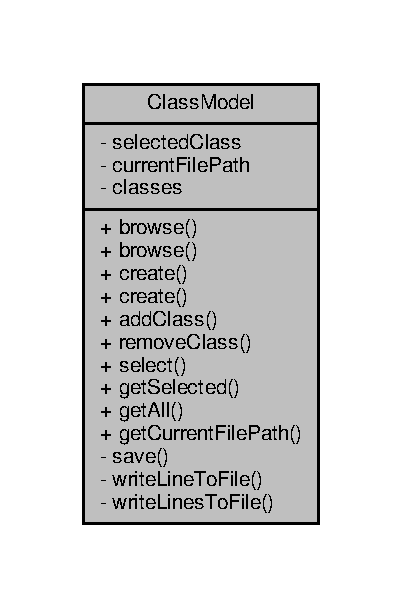
\includegraphics[width=193pt]{classClassModel__coll__graph}
\end{center}
\end{figure}
\subsection*{Public Member Functions}
\begin{DoxyCompactItemize}
\item 
\mbox{\Hypertarget{classClassModel_a275d7d723cceff7cddea637e29bb5489}\label{classClassModel_a275d7d723cceff7cddea637e29bb5489}} 
void \hyperlink{classClassModel_a275d7d723cceff7cddea637e29bb5489}{browse} ()
\begin{DoxyCompactList}\small\item\em Opens a file system dialog window and prompts the user to select a class file. \end{DoxyCompactList}\item 
\mbox{\Hypertarget{classClassModel_a1fb7006db6a2aab398a7c82cab2da568}\label{classClassModel_a1fb7006db6a2aab398a7c82cab2da568}} 
void {\bfseries browse} (const Q\+String \&)
\item 
\mbox{\Hypertarget{classClassModel_afb5c974408ff462e812df971588ea703}\label{classClassModel_afb5c974408ff462e812df971588ea703}} 
void \hyperlink{classClassModel_afb5c974408ff462e812df971588ea703}{create} ()
\begin{DoxyCompactList}\small\item\em Prompts the user for a class file name. Creates a class file using this name. \end{DoxyCompactList}\item 
\mbox{\Hypertarget{classClassModel_ad2e5262948d7491cf1f8bfd305dff829}\label{classClassModel_ad2e5262948d7491cf1f8bfd305dff829}} 
void {\bfseries create} (const Q\+String \&)
\item 
void \hyperlink{classClassModel_ab96bae16ed8f02abf2eca0d7b89a8a62}{add\+Class} (Q\+String)
\begin{DoxyCompactList}\small\item\em Adds a line to the current class file. \end{DoxyCompactList}\item 
void \hyperlink{classClassModel_afe2266d404da4bab25bf193212fed198}{remove\+Class} (const Q\+String \&)
\begin{DoxyCompactList}\small\item\em Removes a line from the current class file. \end{DoxyCompactList}\item 
\mbox{\Hypertarget{classClassModel_a2c8e221161022e6dbe09d07e7fea4422}\label{classClassModel_a2c8e221161022e6dbe09d07e7fea4422}} 
void {\bfseries select} (const std\+::string \&)
\item 
\mbox{\Hypertarget{classClassModel_a935b07226c750dad2410d22fa516db1f}\label{classClassModel_a935b07226c750dad2410d22fa516db1f}} 
std\+::string {\bfseries get\+Selected} ()
\item 
\mbox{\Hypertarget{classClassModel_a0a2c7f3e06cb56c9f3df36c3e8e48031}\label{classClassModel_a0a2c7f3e06cb56c9f3df36c3e8e48031}} 
Q\+String\+List \hyperlink{classClassModel_a0a2c7f3e06cb56c9f3df36c3e8e48031}{get\+All} ()
\begin{DoxyCompactList}\small\item\em Gets a Q\+String\+List of all the classes in the current class file. \end{DoxyCompactList}\item 
\mbox{\Hypertarget{classClassModel_aa952e5109a5246d443f7e83f8a7d75ac}\label{classClassModel_aa952e5109a5246d443f7e83f8a7d75ac}} 
Q\+String \hyperlink{classClassModel_aa952e5109a5246d443f7e83f8a7d75ac}{get\+Current\+File\+Path} ()
\begin{DoxyCompactList}\small\item\em Returns the currently opened file path. \end{DoxyCompactList}\end{DoxyCompactItemize}
\subsection*{Private Member Functions}
\begin{DoxyCompactItemize}
\item 
\mbox{\Hypertarget{classClassModel_ab229a1a8dacc1a892d3757965d6f1e3a}\label{classClassModel_ab229a1a8dacc1a892d3757965d6f1e3a}} 
void {\bfseries save} ()
\item 
void \hyperlink{classClassModel_a4ef5baaf966305d2ebb44bf2c40ee533}{write\+Line\+To\+File} (const Q\+String \&filename, const Q\+String \&line)
\begin{DoxyCompactList}\small\item\em Internal method to write a single line to a file. \end{DoxyCompactList}\item 
void \hyperlink{classClassModel_af78dad5b5b8f214b5067fd1dd629b594}{write\+Lines\+To\+File} (const Q\+String \&filename, const Q\+String\+List \&lines)
\begin{DoxyCompactList}\small\item\em Internal method to write multiple lines to a file. \end{DoxyCompactList}\end{DoxyCompactItemize}
\subsection*{Private Attributes}
\begin{DoxyCompactItemize}
\item 
\mbox{\Hypertarget{classClassModel_a3f55a12cc009fa4a06cd6c82d1ba2a25}\label{classClassModel_a3f55a12cc009fa4a06cd6c82d1ba2a25}} 
std\+::string {\bfseries selected\+Class}
\item 
\mbox{\Hypertarget{classClassModel_a0fbc77cdbd9d9bc73720a83e21b36bc5}\label{classClassModel_a0fbc77cdbd9d9bc73720a83e21b36bc5}} 
Q\+String {\bfseries current\+File\+Path}
\item 
\mbox{\Hypertarget{classClassModel_aa656a0e8e8f9e18a361b427700098405}\label{classClassModel_aa656a0e8e8f9e18a361b427700098405}} 
Q\+String\+List {\bfseries classes}
\end{DoxyCompactItemize}


\subsection{Detailed Description}
\hyperlink{classClassModel}{Class\+Model}, which is responsible for the creating, adding and removing of classes. Maintains internal information about the current selected class and the current file path of the class file. 

\subsection{Member Function Documentation}
\mbox{\Hypertarget{classClassModel_ab96bae16ed8f02abf2eca0d7b89a8a62}\label{classClassModel_ab96bae16ed8f02abf2eca0d7b89a8a62}} 
\index{Class\+Model@{Class\+Model}!add\+Class@{add\+Class}}
\index{add\+Class@{add\+Class}!Class\+Model@{Class\+Model}}
\subsubsection{\texorpdfstring{add\+Class()}{addClass()}}
{\footnotesize\ttfamily void Class\+Model\+::add\+Class (\begin{DoxyParamCaption}\item[{Q\+String}]{class\+Name }\end{DoxyParamCaption})}



Adds a line to the current class file. 

If there is no currently selected class file, the user is prompted by the browse method to select one.


\begin{DoxyParams}{Parameters}
{\em classname} & Name of the class to add. \\
\hline
\end{DoxyParams}
\mbox{\Hypertarget{classClassModel_afe2266d404da4bab25bf193212fed198}\label{classClassModel_afe2266d404da4bab25bf193212fed198}} 
\index{Class\+Model@{Class\+Model}!remove\+Class@{remove\+Class}}
\index{remove\+Class@{remove\+Class}!Class\+Model@{Class\+Model}}
\subsubsection{\texorpdfstring{remove\+Class()}{removeClass()}}
{\footnotesize\ttfamily void Class\+Model\+::remove\+Class (\begin{DoxyParamCaption}\item[{const Q\+String \&}]{class\+Name }\end{DoxyParamCaption})}



Removes a line from the current class file. 

If there is no currently selected class file, the user is promted by the browse method to select one.


\begin{DoxyParams}{Parameters}
{\em classname} & Name of the class to remove. \\
\hline
\end{DoxyParams}
\mbox{\Hypertarget{classClassModel_af78dad5b5b8f214b5067fd1dd629b594}\label{classClassModel_af78dad5b5b8f214b5067fd1dd629b594}} 
\index{Class\+Model@{Class\+Model}!write\+Lines\+To\+File@{write\+Lines\+To\+File}}
\index{write\+Lines\+To\+File@{write\+Lines\+To\+File}!Class\+Model@{Class\+Model}}
\subsubsection{\texorpdfstring{write\+Lines\+To\+File()}{writeLinesToFile()}}
{\footnotesize\ttfamily void Class\+Model\+::write\+Lines\+To\+File (\begin{DoxyParamCaption}\item[{const Q\+String \&}]{file\+Name,  }\item[{const Q\+String\+List \&}]{lines }\end{DoxyParamCaption})\hspace{0.3cm}{\ttfamily [private]}}



Internal method to write multiple lines to a file. 


\begin{DoxyParams}{Parameters}
{\em filename} & File name to write to. \\
\hline
{\em lines} & Lines to write. \\
\hline
\end{DoxyParams}
\mbox{\Hypertarget{classClassModel_a4ef5baaf966305d2ebb44bf2c40ee533}\label{classClassModel_a4ef5baaf966305d2ebb44bf2c40ee533}} 
\index{Class\+Model@{Class\+Model}!write\+Line\+To\+File@{write\+Line\+To\+File}}
\index{write\+Line\+To\+File@{write\+Line\+To\+File}!Class\+Model@{Class\+Model}}
\subsubsection{\texorpdfstring{write\+Line\+To\+File()}{writeLineToFile()}}
{\footnotesize\ttfamily void Class\+Model\+::write\+Line\+To\+File (\begin{DoxyParamCaption}\item[{const Q\+String \&}]{file\+Name,  }\item[{const Q\+String \&}]{line }\end{DoxyParamCaption})\hspace{0.3cm}{\ttfamily [private]}}



Internal method to write a single line to a file. 


\begin{DoxyParams}{Parameters}
{\em filename} & File name to write to. \\
\hline
{\em line} & Line to write. \\
\hline
\end{DoxyParams}


The documentation for this class was generated from the following files\+:\begin{DoxyCompactItemize}
\item 
include/Class\+Model.\+h\item 
src/Class\+Model.\+cpp\end{DoxyCompactItemize}

\hypertarget{classClassNotFoundError}{}\section{Class\+Not\+Found\+Error Class Reference}
\label{classClassNotFoundError}\index{Class\+Not\+Found\+Error@{Class\+Not\+Found\+Error}}


{\ttfamily \#include $<$exceptions.\+h$>$}



Inheritance diagram for Class\+Not\+Found\+Error\+:
\nopagebreak
\begin{figure}[H]
\begin{center}
\leavevmode
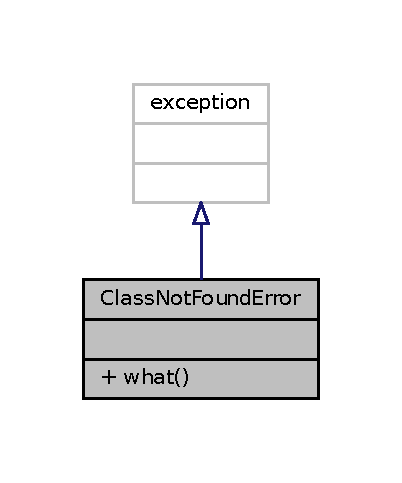
\includegraphics[width=193pt]{classClassNotFoundError__inherit__graph}
\end{center}
\end{figure}


Collaboration diagram for Class\+Not\+Found\+Error\+:
\nopagebreak
\begin{figure}[H]
\begin{center}
\leavevmode
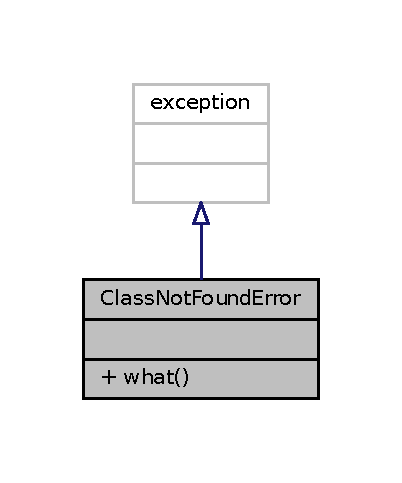
\includegraphics[width=193pt]{classClassNotFoundError__coll__graph}
\end{center}
\end{figure}
\subsection*{Public Member Functions}
\begin{DoxyCompactItemize}
\item 
\mbox{\Hypertarget{classClassNotFoundError_ac3e4abee30e3a59364d93cdf11779345}\label{classClassNotFoundError_ac3e4abee30e3a59364d93cdf11779345}} 
const char $\ast$ {\bfseries what} () const  throw ()
\end{DoxyCompactItemize}


\subsection{Detailed Description}
Custom exception subclass, which signifies a missing class. 

The documentation for this class was generated from the following file\+:\begin{DoxyCompactItemize}
\item 
include/exceptions.\+h\end{DoxyCompactItemize}

\hypertarget{classClassNotSelectedError}{}\section{Class\+Not\+Selected\+Error Class Reference}
\label{classClassNotSelectedError}\index{Class\+Not\+Selected\+Error@{Class\+Not\+Selected\+Error}}


{\ttfamily \#include $<$exceptions.\+h$>$}



Inheritance diagram for Class\+Not\+Selected\+Error\+:
\nopagebreak
\begin{figure}[H]
\begin{center}
\leavevmode
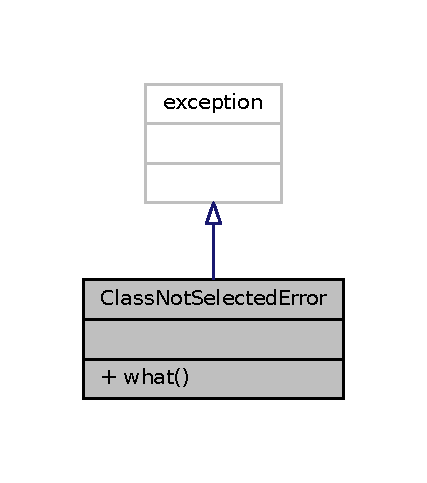
\includegraphics[width=205pt]{classClassNotSelectedError__inherit__graph}
\end{center}
\end{figure}


Collaboration diagram for Class\+Not\+Selected\+Error\+:
\nopagebreak
\begin{figure}[H]
\begin{center}
\leavevmode
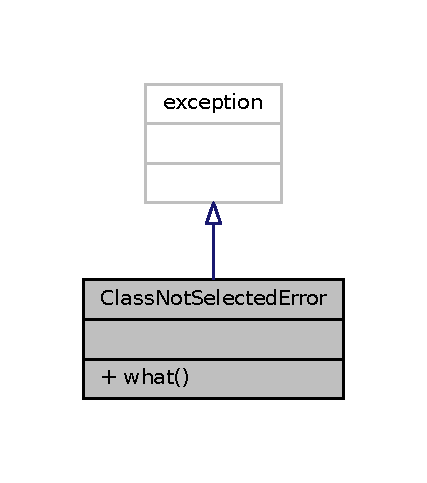
\includegraphics[width=205pt]{classClassNotSelectedError__coll__graph}
\end{center}
\end{figure}
\subsection*{Public Member Functions}
\begin{DoxyCompactItemize}
\item 
\mbox{\Hypertarget{classClassNotSelectedError_a173abddcbffb076d1936b61db9ad46e8}\label{classClassNotSelectedError_a173abddcbffb076d1936b61db9ad46e8}} 
const char $\ast$ {\bfseries what} () const  throw ()
\end{DoxyCompactItemize}


\subsection{Detailed Description}
Custom exception subclass, which signifies that no class is selected. 

The documentation for this class was generated from the following file\+:\begin{DoxyCompactItemize}
\item 
include/exceptions.\+h\end{DoxyCompactItemize}

\hypertarget{classDrawingIncomplete}{}\section{Drawing\+Incomplete Class Reference}
\label{classDrawingIncomplete}\index{Drawing\+Incomplete@{Drawing\+Incomplete}}


{\ttfamily \#include $<$exceptions.\+h$>$}



Inheritance diagram for Drawing\+Incomplete\+:
\nopagebreak
\begin{figure}[H]
\begin{center}
\leavevmode
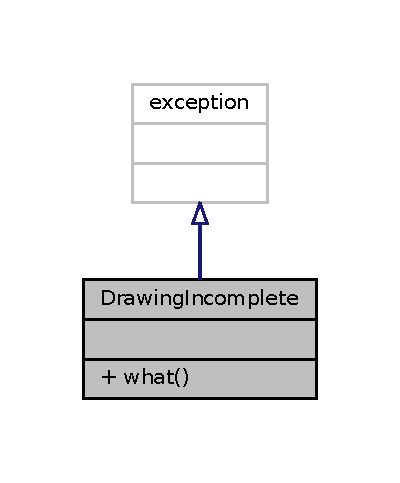
\includegraphics[width=192pt]{classDrawingIncomplete__inherit__graph}
\end{center}
\end{figure}


Collaboration diagram for Drawing\+Incomplete\+:
\nopagebreak
\begin{figure}[H]
\begin{center}
\leavevmode
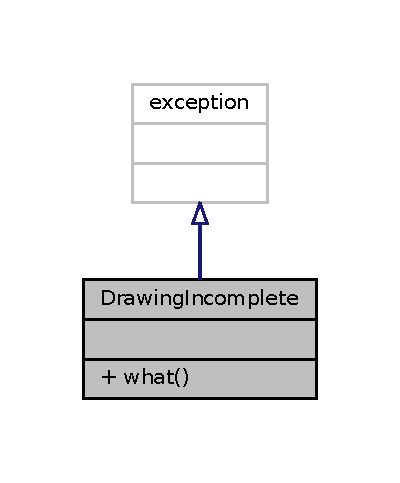
\includegraphics[width=192pt]{classDrawingIncomplete__coll__graph}
\end{center}
\end{figure}
\subsection*{Public Member Functions}
\begin{DoxyCompactItemize}
\item 
\mbox{\Hypertarget{classDrawingIncomplete_afa21aa1cde73e32fee133dbd1b131c3e}\label{classDrawingIncomplete_afa21aa1cde73e32fee133dbd1b131c3e}} 
const char $\ast$ {\bfseries what} () const  throw ()
\end{DoxyCompactItemize}


\subsection{Detailed Description}
Custom exception subclass, which signifies a lack of vertices for a polygon. 

The documentation for this class was generated from the following file\+:\begin{DoxyCompactItemize}
\item 
include/exceptions.\+h\end{DoxyCompactItemize}

\hypertarget{classFileNotFoundError}{}\section{File\+Not\+Found\+Error Class Reference}
\label{classFileNotFoundError}\index{File\+Not\+Found\+Error@{File\+Not\+Found\+Error}}


Inheritance diagram for File\+Not\+Found\+Error\+:
\nopagebreak
\begin{figure}[H]
\begin{center}
\leavevmode
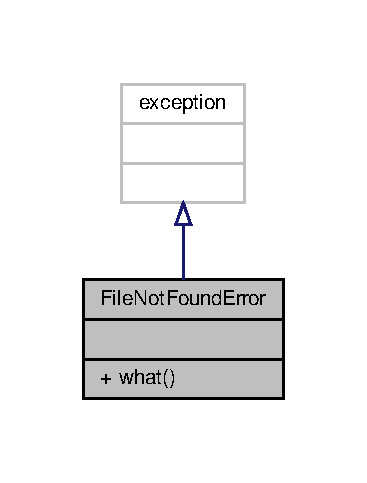
\includegraphics[width=176pt]{classFileNotFoundError__inherit__graph}
\end{center}
\end{figure}


Collaboration diagram for File\+Not\+Found\+Error\+:
\nopagebreak
\begin{figure}[H]
\begin{center}
\leavevmode
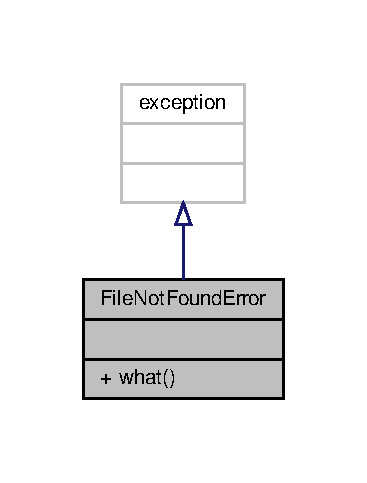
\includegraphics[width=176pt]{classFileNotFoundError__coll__graph}
\end{center}
\end{figure}
\subsection*{Public Member Functions}
\begin{DoxyCompactItemize}
\item 
\mbox{\Hypertarget{classFileNotFoundError_a643cf972753a4adba51d5850cbc619f4}\label{classFileNotFoundError_a643cf972753a4adba51d5850cbc619f4}} 
const char $\ast$ {\bfseries what} () const  throw ()
\end{DoxyCompactItemize}


The documentation for this class was generated from the following file\+:\begin{DoxyCompactItemize}
\item 
include/exceptions.\+h\end{DoxyCompactItemize}

\hypertarget{classFolderNotFoundError}{}\section{Folder\+Not\+Found\+Error Class Reference}
\label{classFolderNotFoundError}\index{Folder\+Not\+Found\+Error@{Folder\+Not\+Found\+Error}}


{\ttfamily \#include $<$exceptions.\+h$>$}



Inheritance diagram for Folder\+Not\+Found\+Error\+:\nopagebreak
\begin{figure}[H]
\begin{center}
\leavevmode
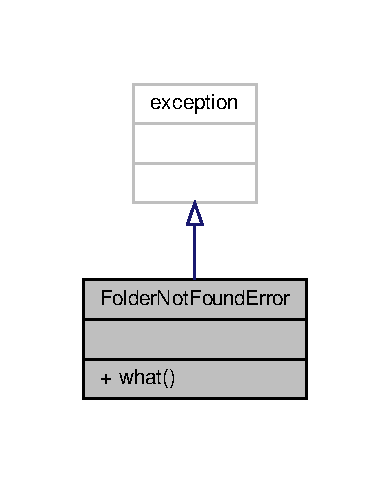
\includegraphics[width=187pt]{classFolderNotFoundError__inherit__graph}
\end{center}
\end{figure}


Collaboration diagram for Folder\+Not\+Found\+Error\+:\nopagebreak
\begin{figure}[H]
\begin{center}
\leavevmode
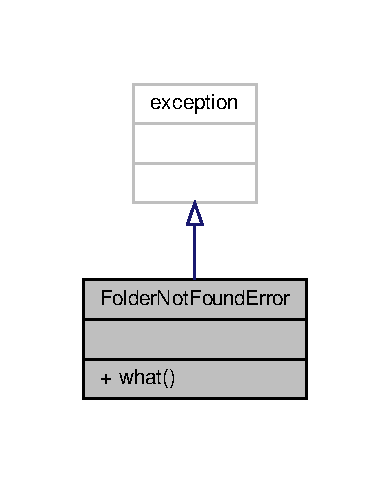
\includegraphics[width=187pt]{classFolderNotFoundError__coll__graph}
\end{center}
\end{figure}
\subsection*{Public Member Functions}
\begin{DoxyCompactItemize}
\item 
\mbox{\Hypertarget{classFolderNotFoundError_a241dcd046686f65f53bbd4c5a7c21ac5}\label{classFolderNotFoundError_a241dcd046686f65f53bbd4c5a7c21ac5}} 
const char $\ast$ {\bfseries what} () const  throw ()
\end{DoxyCompactItemize}


\subsection{Detailed Description}
Custom exception subclass, which signifies a missing folder. 

The documentation for this class was generated from the following file\+:\begin{DoxyCompactItemize}
\item 
include/exceptions.\+h\end{DoxyCompactItemize}

\hypertarget{classGraphicsView}{}\section{Graphics\+View Class Reference}
\label{classGraphicsView}\index{Graphics\+View@{Graphics\+View}}


Inheritance diagram for Graphics\+View\+:
\nopagebreak
\begin{figure}[H]
\begin{center}
\leavevmode
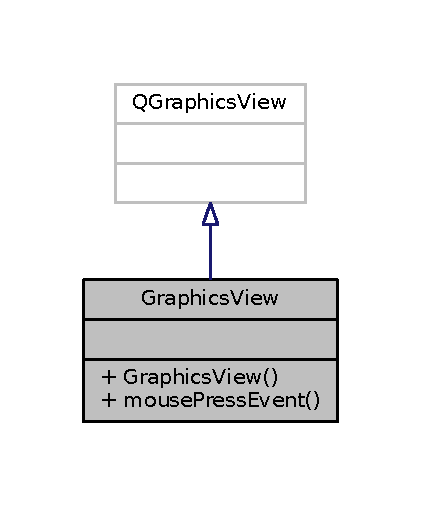
\includegraphics[width=202pt]{classGraphicsView__inherit__graph}
\end{center}
\end{figure}


Collaboration diagram for Graphics\+View\+:
\nopagebreak
\begin{figure}[H]
\begin{center}
\leavevmode
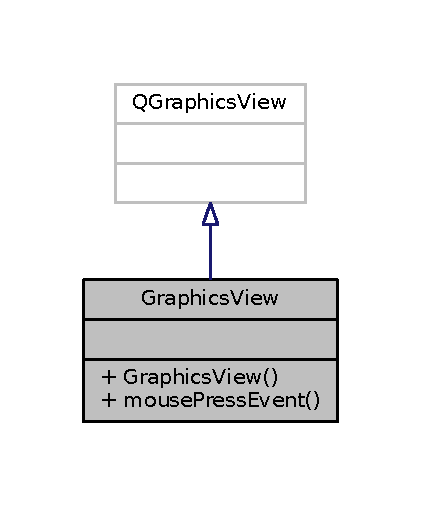
\includegraphics[width=202pt]{classGraphicsView__coll__graph}
\end{center}
\end{figure}
\subsection*{Signals}
\begin{DoxyCompactItemize}
\item 
\mbox{\Hypertarget{classGraphicsView_a714015685be9eb1b83cee3090fce8040}\label{classGraphicsView_a714015685be9eb1b83cee3090fce8040}} 
void {\bfseries send\+Mouse\+Position} (Q\+Point)
\end{DoxyCompactItemize}
\subsection*{Public Member Functions}
\begin{DoxyCompactItemize}
\item 
\mbox{\Hypertarget{classGraphicsView_a0d9eb9dcb2de6db21b054c9afa45c35b}\label{classGraphicsView_a0d9eb9dcb2de6db21b054c9afa45c35b}} 
{\bfseries Graphics\+View} (Q\+Widget $\ast$)
\item 
\mbox{\Hypertarget{classGraphicsView_a8d9cb599e552ae981ed0d0f10ebf4b63}\label{classGraphicsView_a8d9cb599e552ae981ed0d0f10ebf4b63}} 
void {\bfseries mouse\+Press\+Event} (Q\+Mouse\+Event $\ast$event)
\end{DoxyCompactItemize}


The documentation for this class was generated from the following files\+:\begin{DoxyCompactItemize}
\item 
include/Graphics\+View.\+h\item 
src/Graphics\+View.\+cpp\end{DoxyCompactItemize}

\hypertarget{classImageController}{}\section{Image\+Controller Class Reference}
\label{classImageController}\index{Image\+Controller@{Image\+Controller}}


{\ttfamily \#include $<$Image\+Controller.\+h$>$}



Collaboration diagram for Image\+Controller\+:\nopagebreak
\begin{figure}[H]
\begin{center}
\leavevmode
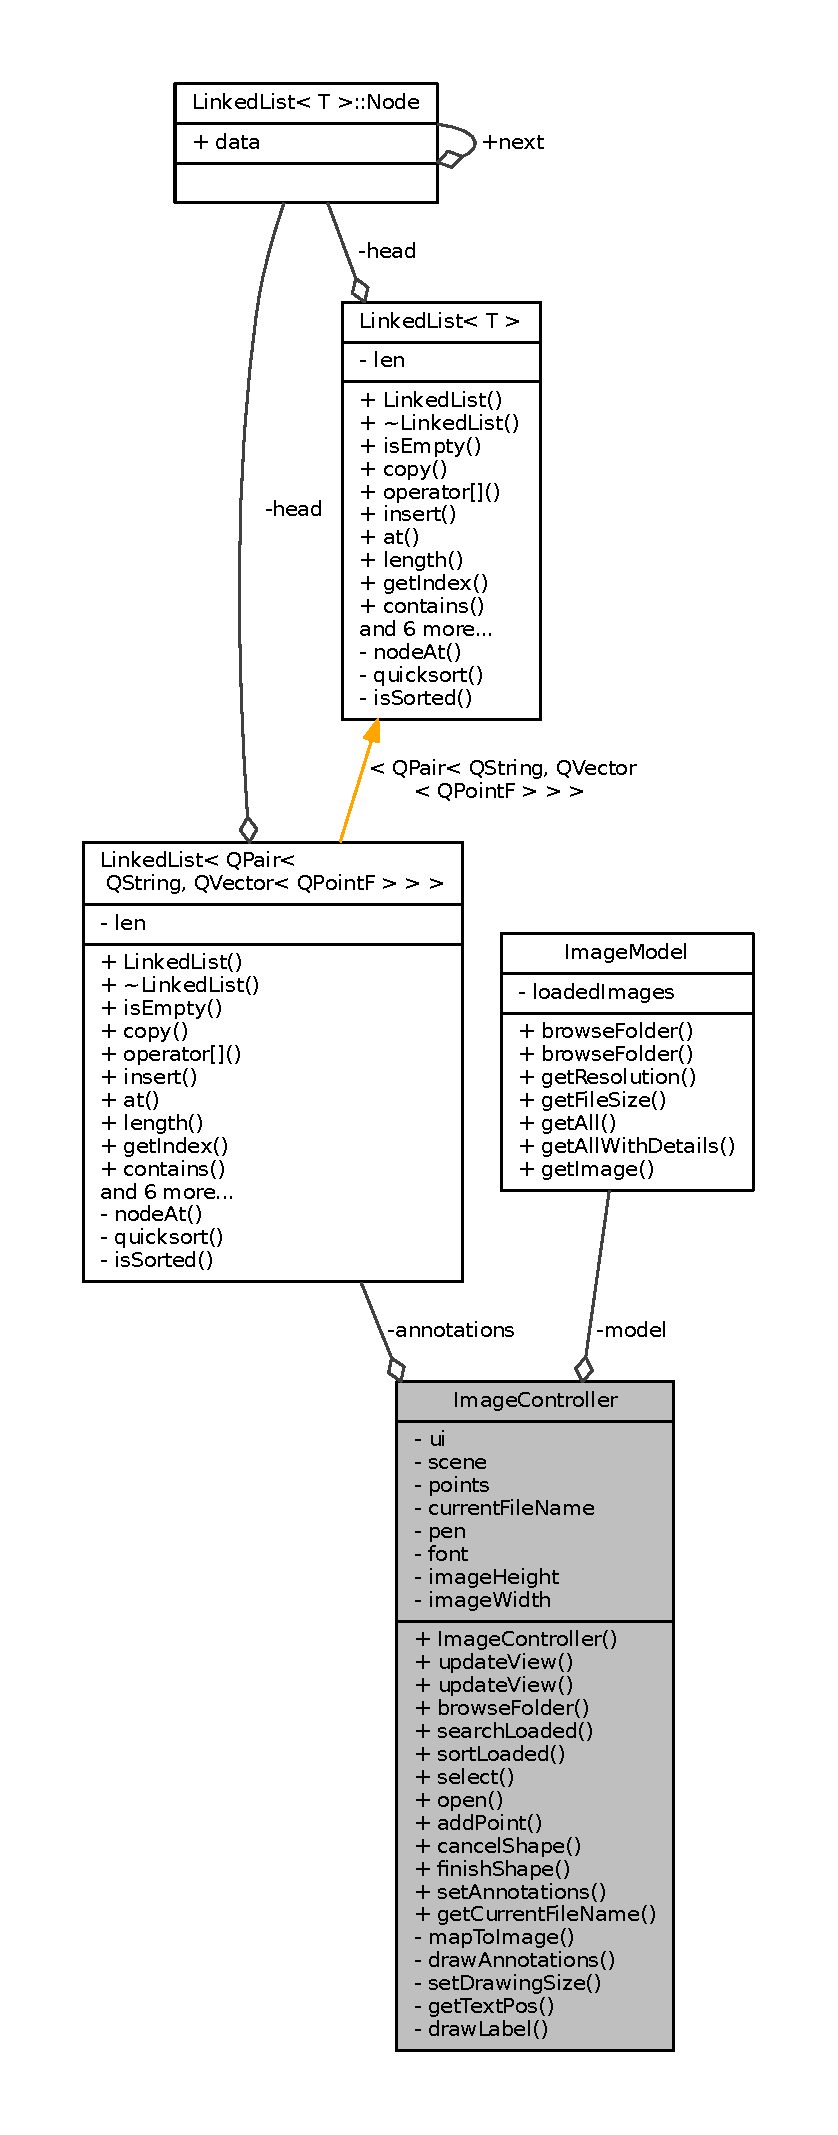
\includegraphics[width=181pt]{classImageController__coll__graph}
\end{center}
\end{figure}
\subsection*{Public Member Functions}
\begin{DoxyCompactItemize}
\item 
\hyperlink{classImageController_a317e49c29f50578a1001b73749151e3a}{Image\+Controller} (Ui\+\_\+\+Main\+View \&, \hyperlink{classImageModel}{Image\+Model} \&)
\begin{DoxyCompactList}\small\item\em Constructs an \hyperlink{classImageController}{Image\+Controller}, which handles business logic, related to the image files. \end{DoxyCompactList}\item 
\mbox{\Hypertarget{classImageController_a203590172b061a2e20d09dc9f8f060b7}\label{classImageController_a203590172b061a2e20d09dc9f8f060b7}} 
void \hyperlink{classImageController_a203590172b061a2e20d09dc9f8f060b7}{browse\+Folder} ()
\begin{DoxyCompactList}\small\item\em Browses for a new folder containing images, then updates the view to reflect that. \end{DoxyCompactList}\item 
\mbox{\Hypertarget{classImageController_a29879b8ce218c266f100ef6da70687ca}\label{classImageController_a29879b8ce218c266f100ef6da70687ca}} 
void {\bfseries search\+Loaded} (const Q\+String \&)
\item 
\mbox{\Hypertarget{classImageController_aa27c122f5fa43ed32984077cc0f1871a}\label{classImageController_aa27c122f5fa43ed32984077cc0f1871a}} 
void {\bfseries sort\+Loaded} ()
\item 
\mbox{\Hypertarget{classImageController_a81d44568235778fe6d5dc14fb377499a}\label{classImageController_a81d44568235778fe6d5dc14fb377499a}} 
void {\bfseries select} (const Q\+String \&)
\item 
void \hyperlink{classImageController_a3f5976d87977aa1cda7b5a9a7ad0f03b}{open} (const Q\+String \&)
\begin{DoxyCompactList}\small\item\em Gets a filename from the Main\+Controler, opens image and displays it in the \hyperlink{classMainView}{Main\+View}. \end{DoxyCompactList}\end{DoxyCompactItemize}
\subsection*{Private Member Functions}
\begin{DoxyCompactItemize}
\item 
\mbox{\Hypertarget{classImageController_a3a300727ff5e30b19fcc0102427fdb30}\label{classImageController_a3a300727ff5e30b19fcc0102427fdb30}} 
void \hyperlink{classImageController_a3a300727ff5e30b19fcc0102427fdb30}{update\+View} ()
\begin{DoxyCompactList}\small\item\em Clears the list of loaded images in the G\+UI and refills them from the currently loaded images. \end{DoxyCompactList}\end{DoxyCompactItemize}
\subsection*{Private Attributes}
\begin{DoxyCompactItemize}
\item 
\mbox{\Hypertarget{classImageController_ac4a8d61dbfe0c1a0b63f7cd456b3c1c1}\label{classImageController_ac4a8d61dbfe0c1a0b63f7cd456b3c1c1}} 
Ui\+\_\+\+Main\+View {\bfseries ui}
\item 
\mbox{\Hypertarget{classImageController_a7b83dbab8de169f4c1d394a72280aec5}\label{classImageController_a7b83dbab8de169f4c1d394a72280aec5}} 
\hyperlink{classImageModel}{Image\+Model} {\bfseries model}
\end{DoxyCompactItemize}


\subsection{Detailed Description}
Sub-\/controller, which gets delegated tasks, relating to loading, storing and updating images. Communicates directly with the \hyperlink{classImageModel}{Image\+Model}. 

\subsection{Constructor \& Destructor Documentation}
\mbox{\Hypertarget{classImageController_a317e49c29f50578a1001b73749151e3a}\label{classImageController_a317e49c29f50578a1001b73749151e3a}} 
\index{Image\+Controller@{Image\+Controller}!Image\+Controller@{Image\+Controller}}
\index{Image\+Controller@{Image\+Controller}!Image\+Controller@{Image\+Controller}}
\subsubsection{\texorpdfstring{Image\+Controller()}{ImageController()}}
{\footnotesize\ttfamily Image\+Controller\+::\+Image\+Controller (\begin{DoxyParamCaption}\item[{Ui\+\_\+\+Main\+View \&}]{ui,  }\item[{\hyperlink{classImageModel}{Image\+Model} \&}]{model }\end{DoxyParamCaption})}



Constructs an \hyperlink{classImageController}{Image\+Controller}, which handles business logic, related to the image files. 


\begin{DoxyParams}{Parameters}
{\em ui} & The Ui\+\_\+\+Main\+View reference, which is used to update the G\+UI. \\
\hline
{\em model} & \\
\hline
\end{DoxyParams}


\subsection{Member Function Documentation}
\mbox{\Hypertarget{classImageController_a3f5976d87977aa1cda7b5a9a7ad0f03b}\label{classImageController_a3f5976d87977aa1cda7b5a9a7ad0f03b}} 
\index{Image\+Controller@{Image\+Controller}!open@{open}}
\index{open@{open}!Image\+Controller@{Image\+Controller}}
\subsubsection{\texorpdfstring{open()}{open()}}
{\footnotesize\ttfamily void Image\+Controller\+::open (\begin{DoxyParamCaption}\item[{const Q\+String \&}]{file\+Name }\end{DoxyParamCaption})}



Gets a filename from the Main\+Controler, opens image and displays it in the \hyperlink{classMainView}{Main\+View}. 


\begin{DoxyParams}{Parameters}
{\em filename} & \\
\hline
\end{DoxyParams}


The documentation for this class was generated from the following files\+:\begin{DoxyCompactItemize}
\item 
include/Image\+Controller.\+h\item 
src/Image\+Controller.\+cpp\end{DoxyCompactItemize}

\hypertarget{classImageModel}{}\section{Image\+Model Class Reference}
\label{classImageModel}\index{Image\+Model@{Image\+Model}}


{\ttfamily \#include $<$Image\+Model.\+h$>$}



Collaboration diagram for Image\+Model\+:
\nopagebreak
\begin{figure}[H]
\begin{center}
\leavevmode
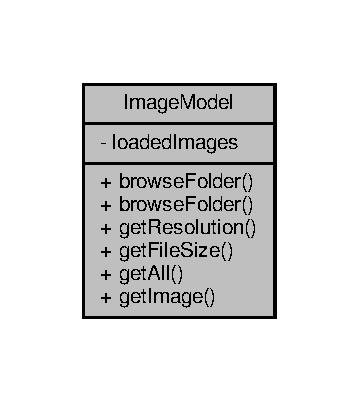
\includegraphics[width=172pt]{classImageModel__coll__graph}
\end{center}
\end{figure}
\subsection*{Public Member Functions}
\begin{DoxyCompactItemize}
\item 
\mbox{\Hypertarget{classImageModel_a556093e64b3d118525120e465a7dedf6}\label{classImageModel_a556093e64b3d118525120e465a7dedf6}} 
void \hyperlink{classImageModel_a556093e64b3d118525120e465a7dedf6}{browse\+Folder} ()
\begin{DoxyCompactList}\small\item\em Opens a system file dialog window and promps the user for an image folder. \end{DoxyCompactList}\item 
void \hyperlink{classImageModel_a4923192da890831266d2348ce54b2e45}{browse\+Folder} (const Q\+String \&)
\begin{DoxyCompactList}\small\item\em Provides a way to input folder path to the system without loading up the G\+UI. \end{DoxyCompactList}\item 
std\+::pair$<$ int, int $>$ \hyperlink{classImageModel_af44b02e6974b36d2ede3b1b3f78ebc84}{get\+Resolution} (const Q\+String \&)
\begin{DoxyCompactList}\small\item\em Provides a way to read resolution of a given image file. \end{DoxyCompactList}\item 
long \hyperlink{classImageModel_a38c8d5868b7a8f8acca235c4383c5102}{get\+File\+Size} (const Q\+String \&)
\begin{DoxyCompactList}\small\item\em Provides a way to read file size of a given image file. \end{DoxyCompactList}\item 
Q\+String\+List \hyperlink{classImageModel_a498623ffa9423fd249c62467c01edeee}{get\+All} ()
\begin{DoxyCompactList}\small\item\em Returns all loaded images in the \hyperlink{classImageModel}{Image\+Model}. \end{DoxyCompactList}\item 
Q\+Image \hyperlink{classImageModel_ac0021794e5694bd76c76349b8af96428}{get\+Image} (const Q\+String \&)
\begin{DoxyCompactList}\small\item\em Provides a way to get an actual image from the system. \end{DoxyCompactList}\end{DoxyCompactItemize}
\subsection*{Private Attributes}
\begin{DoxyCompactItemize}
\item 
\mbox{\Hypertarget{classImageModel_a238323b509f2644dcd2858558a40448a}\label{classImageModel_a238323b509f2644dcd2858558a40448a}} 
Q\+Map$<$ Q\+String, Q\+File\+Info $>$ {\bfseries loaded\+Images}
\end{DoxyCompactItemize}


\subsection{Detailed Description}
Model, which is responsible for file handling of images. Maintains an internal list of the currently loaded images. 

\subsection{Member Function Documentation}
\mbox{\Hypertarget{classImageModel_a4923192da890831266d2348ce54b2e45}\label{classImageModel_a4923192da890831266d2348ce54b2e45}} 
\index{Image\+Model@{Image\+Model}!browse\+Folder@{browse\+Folder}}
\index{browse\+Folder@{browse\+Folder}!Image\+Model@{Image\+Model}}
\subsubsection{\texorpdfstring{browse\+Folder()}{browseFolder()}}
{\footnotesize\ttfamily void Image\+Model\+::browse\+Folder (\begin{DoxyParamCaption}\item[{const Q\+String \&}]{folder\+Path }\end{DoxyParamCaption})}



Provides a way to input folder path to the system without loading up the G\+UI. 


\begin{DoxyParams}{Parameters}
{\em Path} & to a folder user wants to browse \\
\hline
\end{DoxyParams}
\mbox{\Hypertarget{classImageModel_a498623ffa9423fd249c62467c01edeee}\label{classImageModel_a498623ffa9423fd249c62467c01edeee}} 
\index{Image\+Model@{Image\+Model}!get\+All@{get\+All}}
\index{get\+All@{get\+All}!Image\+Model@{Image\+Model}}
\subsubsection{\texorpdfstring{get\+All()}{getAll()}}
{\footnotesize\ttfamily Q\+String\+List Image\+Model\+::get\+All (\begin{DoxyParamCaption}{ }\end{DoxyParamCaption})}



Returns all loaded images in the \hyperlink{classImageModel}{Image\+Model}. 

\begin{DoxyReturn}{Returns}
Q\+String\+List for every loaded image 
\end{DoxyReturn}
\mbox{\Hypertarget{classImageModel_a38c8d5868b7a8f8acca235c4383c5102}\label{classImageModel_a38c8d5868b7a8f8acca235c4383c5102}} 
\index{Image\+Model@{Image\+Model}!get\+File\+Size@{get\+File\+Size}}
\index{get\+File\+Size@{get\+File\+Size}!Image\+Model@{Image\+Model}}
\subsubsection{\texorpdfstring{get\+File\+Size()}{getFileSize()}}
{\footnotesize\ttfamily long Image\+Model\+::get\+File\+Size (\begin{DoxyParamCaption}\item[{const Q\+String \&}]{file\+Name }\end{DoxyParamCaption})}



Provides a way to read file size of a given image file. 


\begin{DoxyParams}{Parameters}
{\em Name} & of a image file \\
\hline
\end{DoxyParams}
\begin{DoxyReturn}{Returns}
File size of image, in bytes 
\end{DoxyReturn}
\mbox{\Hypertarget{classImageModel_ac0021794e5694bd76c76349b8af96428}\label{classImageModel_ac0021794e5694bd76c76349b8af96428}} 
\index{Image\+Model@{Image\+Model}!get\+Image@{get\+Image}}
\index{get\+Image@{get\+Image}!Image\+Model@{Image\+Model}}
\subsubsection{\texorpdfstring{get\+Image()}{getImage()}}
{\footnotesize\ttfamily Q\+Image Image\+Model\+::get\+Image (\begin{DoxyParamCaption}\item[{const Q\+String \&}]{filename }\end{DoxyParamCaption})}



Provides a way to get an actual image from the system. 

Gets name of the image from \hyperlink{classImageController}{Image\+Controller}, searches for file path using image file name from internal map. After that it creates Image object and returns it to \hyperlink{classImageController}{Image\+Controller}


\begin{DoxyParams}{Parameters}
{\em Name} & of a image file \\
\hline
\end{DoxyParams}
\begin{DoxyReturn}{Returns}
Q\+Image of image provided via image filename 
\end{DoxyReturn}
\mbox{\Hypertarget{classImageModel_af44b02e6974b36d2ede3b1b3f78ebc84}\label{classImageModel_af44b02e6974b36d2ede3b1b3f78ebc84}} 
\index{Image\+Model@{Image\+Model}!get\+Resolution@{get\+Resolution}}
\index{get\+Resolution@{get\+Resolution}!Image\+Model@{Image\+Model}}
\subsubsection{\texorpdfstring{get\+Resolution()}{getResolution()}}
{\footnotesize\ttfamily std\+::pair$<$ int, int $>$ Image\+Model\+::get\+Resolution (\begin{DoxyParamCaption}\item[{const Q\+String \&}]{file\+Name }\end{DoxyParamCaption})}



Provides a way to read resolution of a given image file. 


\begin{DoxyParams}{Parameters}
{\em Name} & of a image file \\
\hline
\end{DoxyParams}
\begin{DoxyReturn}{Returns}
std\+::pair of image resolution, in format $<$x,y$>$ 
\end{DoxyReturn}


The documentation for this class was generated from the following files\+:\begin{DoxyCompactItemize}
\item 
include/Image\+Model.\+h\item 
src/Image\+Model.\+cpp\end{DoxyCompactItemize}

\hypertarget{classImageNotAnnotatedYet}{}\section{Image\+Not\+Annotated\+Yet Class Reference}
\label{classImageNotAnnotatedYet}\index{Image\+Not\+Annotated\+Yet@{Image\+Not\+Annotated\+Yet}}


{\ttfamily \#include $<$exceptions.\+h$>$}



Inheritance diagram for Image\+Not\+Annotated\+Yet\+:\nopagebreak
\begin{figure}[H]
\begin{center}
\leavevmode
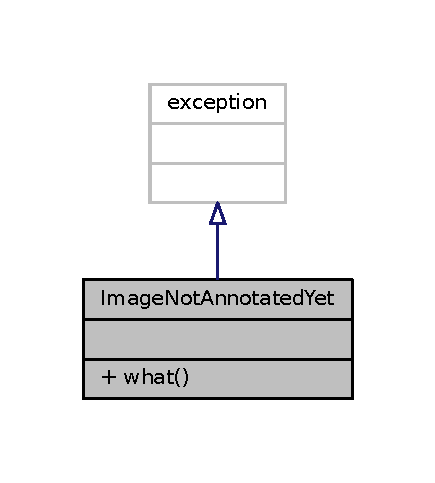
\includegraphics[width=209pt]{classImageNotAnnotatedYet__inherit__graph}
\end{center}
\end{figure}


Collaboration diagram for Image\+Not\+Annotated\+Yet\+:\nopagebreak
\begin{figure}[H]
\begin{center}
\leavevmode
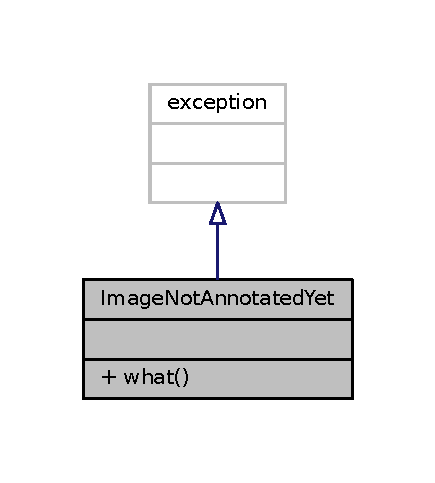
\includegraphics[width=209pt]{classImageNotAnnotatedYet__coll__graph}
\end{center}
\end{figure}
\subsection*{Public Member Functions}
\begin{DoxyCompactItemize}
\item 
\mbox{\Hypertarget{classImageNotAnnotatedYet_a092756a54b3f53ff6026bfc150e6fc8c}\label{classImageNotAnnotatedYet_a092756a54b3f53ff6026bfc150e6fc8c}} 
const char $\ast$ {\bfseries what} () const  throw ()
\end{DoxyCompactItemize}


\subsection{Detailed Description}
Custom exception subclass, which signifies an image, which hasn\textquotesingle{}t been annotated yet. 

The documentation for this class was generated from the following file\+:\begin{DoxyCompactItemize}
\item 
include/exceptions.\+h\end{DoxyCompactItemize}

\hypertarget{classIndexOutOfBoundsError}{}\section{Index\+Out\+Of\+Bounds\+Error Class Reference}
\label{classIndexOutOfBoundsError}\index{Index\+Out\+Of\+Bounds\+Error@{Index\+Out\+Of\+Bounds\+Error}}


{\ttfamily \#include $<$exceptions.\+h$>$}



Inheritance diagram for Index\+Out\+Of\+Bounds\+Error\+:\nopagebreak
\begin{figure}[H]
\begin{center}
\leavevmode
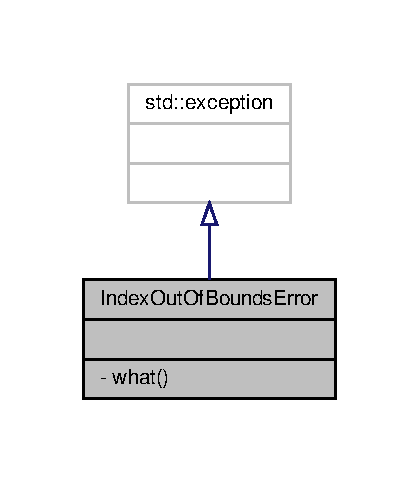
\includegraphics[width=201pt]{classIndexOutOfBoundsError__inherit__graph}
\end{center}
\end{figure}


Collaboration diagram for Index\+Out\+Of\+Bounds\+Error\+:\nopagebreak
\begin{figure}[H]
\begin{center}
\leavevmode
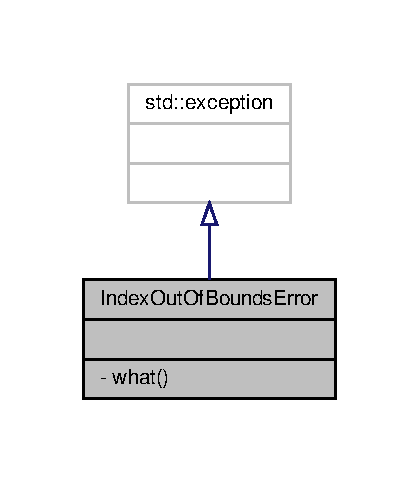
\includegraphics[width=201pt]{classIndexOutOfBoundsError__coll__graph}
\end{center}
\end{figure}
\subsection*{Private Member Functions}
\begin{DoxyCompactItemize}
\item 
\mbox{\Hypertarget{classIndexOutOfBoundsError_a9077c8657e9bd2bd2d42d3d74b9770b6}\label{classIndexOutOfBoundsError_a9077c8657e9bd2bd2d42d3d74b9770b6}} 
const char $\ast$ {\bfseries what} () const  throw ()
\end{DoxyCompactItemize}


\subsection{Detailed Description}
Custom exception subclass, which signifies an array index out of bounds. 

The documentation for this class was generated from the following file\+:\begin{DoxyCompactItemize}
\item 
include/exceptions.\+h\end{DoxyCompactItemize}

\hypertarget{classLinkedList}{}\section{Linked\+List$<$ T $>$ Class Template Reference}
\label{classLinkedList}\index{Linked\+List$<$ T $>$@{Linked\+List$<$ T $>$}}


{\ttfamily \#include $<$Linked\+List.\+h$>$}



Inheritance diagram for Linked\+List$<$ T $>$\+:
\nopagebreak
\begin{figure}[H]
\begin{center}
\leavevmode
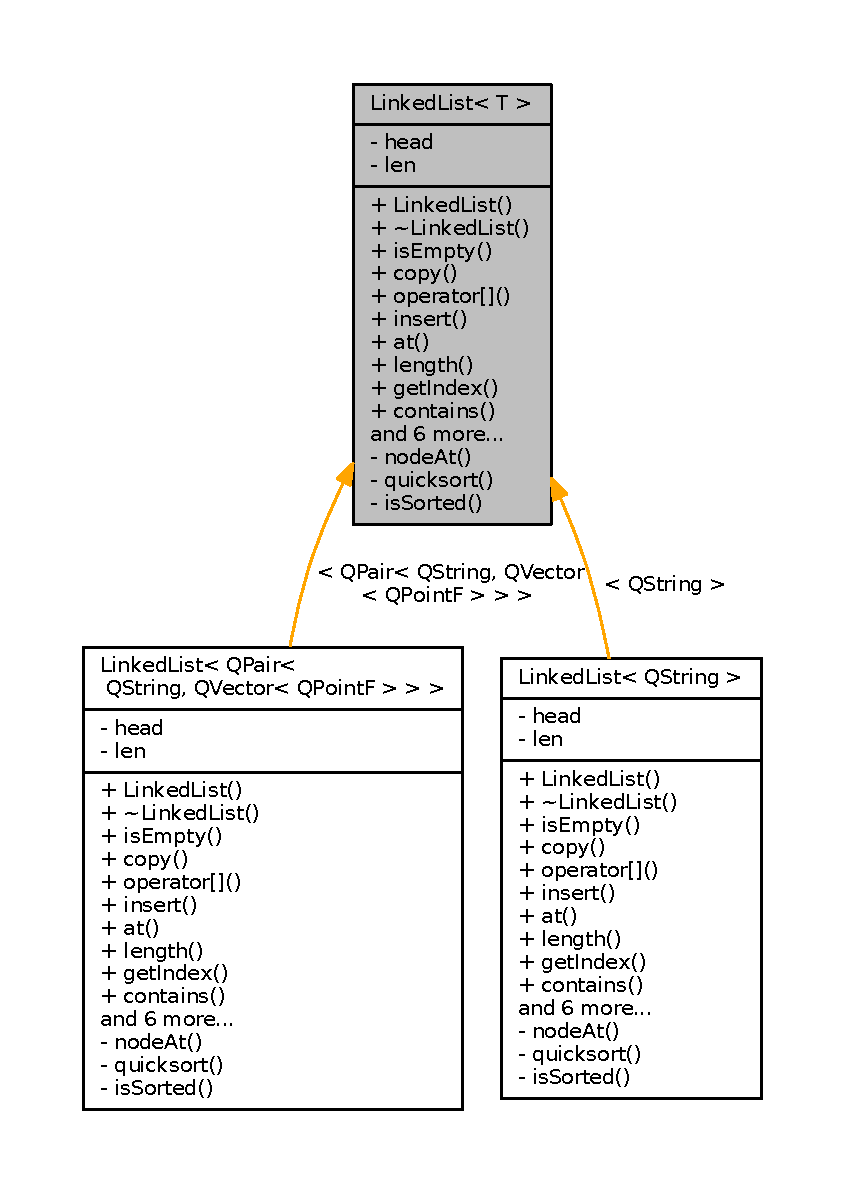
\includegraphics[width=350pt]{classLinkedList__inherit__graph}
\end{center}
\end{figure}


Collaboration diagram for Linked\+List$<$ T $>$\+:
\nopagebreak
\begin{figure}[H]
\begin{center}
\leavevmode
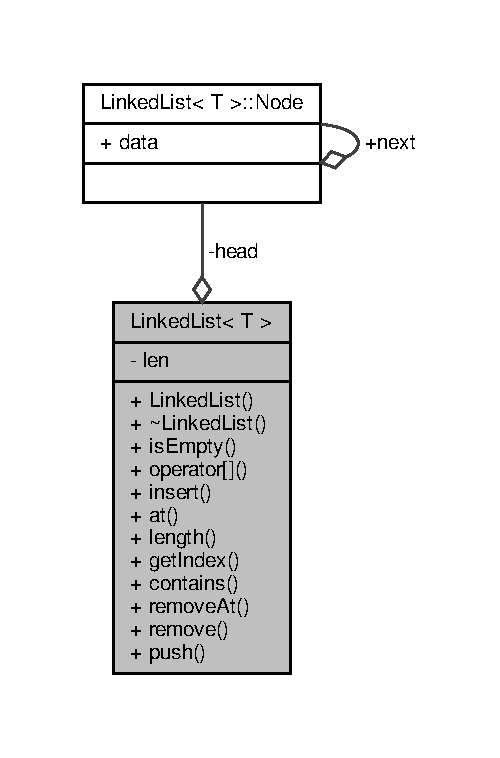
\includegraphics[width=258pt]{classLinkedList__coll__graph}
\end{center}
\end{figure}
\subsection*{Classes}
\begin{DoxyCompactItemize}
\item 
struct \hyperlink{structLinkedList_1_1Node}{Node}
\end{DoxyCompactItemize}
\subsection*{Public Member Functions}
\begin{DoxyCompactItemize}
\item 
\mbox{\Hypertarget{classLinkedList_a3c20fcfec867e867f541061a09fc640c}\label{classLinkedList_a3c20fcfec867e867f541061a09fc640c}} 
\hyperlink{classLinkedList_a3c20fcfec867e867f541061a09fc640c}{Linked\+List} ()
\begin{DoxyCompactList}\small\item\em \hyperlink{classLinkedList}{Linked\+List} Constructor for an empty list. \end{DoxyCompactList}\item 
bool \hyperlink{classLinkedList_a7ecbb28e82117a680839ed0dc28ebdce}{is\+Empty} ()
\begin{DoxyCompactList}\small\item\em Checks if the list is empty. \end{DoxyCompactList}\item 
\hyperlink{classLinkedList}{Linked\+List} \hyperlink{classLinkedList_aadd88559a0e7e92c6a7da3e117b4e26f}{copy} ()
\begin{DoxyCompactList}\small\item\em Creates copy of this linked list. \end{DoxyCompactList}\item 
T \hyperlink{classLinkedList_a83a2aadda160e4f1160b35fd64f72207}{operator\mbox{[}$\,$\mbox{]}} (size\+\_\+t index)
\begin{DoxyCompactList}\small\item\em Gets the data of the node at the index specified. \end{DoxyCompactList}\item 
\hyperlink{structLinkedList_1_1Node}{Node} $\ast$ \hyperlink{classLinkedList_ae5e1ea8a9bbb18d9483db99b44479566}{insert} (size\+\_\+t index, T data)
\begin{DoxyCompactList}\small\item\em Inserts a new node. \end{DoxyCompactList}\item 
T \hyperlink{classLinkedList_a2793ba03677f44075c0529dffe0b0d5a}{at} (size\+\_\+t index)
\begin{DoxyCompactList}\small\item\em Gets the data of the node at the index specified. \end{DoxyCompactList}\item 
size\+\_\+t \hyperlink{classLinkedList_a4b766729a31801b6fafdb6170646d318}{length} ()
\begin{DoxyCompactList}\small\item\em Gets the length of the list. \end{DoxyCompactList}\item 
size\+\_\+t \hyperlink{classLinkedList_ac274901e769cff00d61b52844e96b21e}{get\+Index} (T data)
\begin{DoxyCompactList}\small\item\em Returns the index of the first node with the given data. \end{DoxyCompactList}\item 
bool \hyperlink{classLinkedList_a603e1c5a0a4528d82f83b9393f83bf22}{contains} (T data)
\begin{DoxyCompactList}\small\item\em Checks if the list contains a node with the given data. \end{DoxyCompactList}\item 
void \hyperlink{classLinkedList_ae19893f875003b17caf0f71d26167fd4}{remove\+At} (size\+\_\+t index)
\begin{DoxyCompactList}\small\item\em Removes the node at the given index. \end{DoxyCompactList}\item 
void \hyperlink{classLinkedList_ab9aa6e03f271785f6b488d8c4cc3f3c7}{remove} (T data)
\begin{DoxyCompactList}\small\item\em Removes the first node with the given data. \end{DoxyCompactList}\item 
void \hyperlink{classLinkedList_a0a7ce2592ff7566349f68a1cb60bf00b}{replace} (size\+\_\+t index, T data)
\begin{DoxyCompactList}\small\item\em replace Replace a node\textquotesingle{}s data. \end{DoxyCompactList}\item 
\hyperlink{structLinkedList_1_1Node}{Node} $\ast$ \hyperlink{classLinkedList_a3a1e6c2009b611fb4416574178b316a3}{push} (T data)
\begin{DoxyCompactList}\small\item\em Inserts a new node to the end of the list. \end{DoxyCompactList}\item 
\mbox{\Hypertarget{classLinkedList_a691b27f81c60be3c891fe6d56a4718b4}\label{classLinkedList_a691b27f81c60be3c891fe6d56a4718b4}} 
void \hyperlink{classLinkedList_a691b27f81c60be3c891fe6d56a4718b4}{sort} ()
\begin{DoxyCompactList}\small\item\em Sorts the linked list in-\/place. \end{DoxyCompactList}\item 
\mbox{\Hypertarget{classLinkedList_a50c26292740c964ac7bef0e072868be1}\label{classLinkedList_a50c26292740c964ac7bef0e072868be1}} 
void \hyperlink{classLinkedList_a50c26292740c964ac7bef0e072868be1}{clear} ()
\begin{DoxyCompactList}\small\item\em clear Clears the linked list. \end{DoxyCompactList}\end{DoxyCompactItemize}
\subsection*{Private Member Functions}
\begin{DoxyCompactItemize}
\item 
\hyperlink{structLinkedList_1_1Node}{Node} $\ast$ \hyperlink{classLinkedList_ae19ff3c4e501a9638fa5caf5cc9d5b05}{node\+At} (size\+\_\+t index)
\begin{DoxyCompactList}\small\item\em node\+At Returns the node at the specified index. \end{DoxyCompactList}\item 
void \hyperlink{classLinkedList_a38612b71d816fec54ea379d0b8daec76}{quicksort} (size\+\_\+t left, size\+\_\+t right)
\begin{DoxyCompactList}\small\item\em An internal implementation of the quicksort algorithm. \end{DoxyCompactList}\item 
bool \hyperlink{classLinkedList_ae7e96c18033f13a7ddb22a4b5ba4cc7e}{is\+Sorted} ()
\begin{DoxyCompactList}\small\item\em Checks if a list is sorted. \end{DoxyCompactList}\end{DoxyCompactItemize}
\subsection*{Private Attributes}
\begin{DoxyCompactItemize}
\item 
\mbox{\Hypertarget{classLinkedList_a2d1f848e19caa3f180b7fa6938125bba}\label{classLinkedList_a2d1f848e19caa3f180b7fa6938125bba}} 
\hyperlink{structLinkedList_1_1Node}{Node} $\ast$ {\bfseries head}
\item 
\mbox{\Hypertarget{classLinkedList_a61a7fe2947bd2d1dbf09a9a97bf7b3ce}\label{classLinkedList_a61a7fe2947bd2d1dbf09a9a97bf7b3ce}} 
size\+\_\+t {\bfseries len} \{0\}
\end{DoxyCompactItemize}


\subsection{Detailed Description}
\subsubsection*{template$<$class T$>$\newline
class Linked\+List$<$ T $>$}

Custom implementation of a singly-\/linked list. 

\subsection{Member Function Documentation}
\mbox{\Hypertarget{classLinkedList_a2793ba03677f44075c0529dffe0b0d5a}\label{classLinkedList_a2793ba03677f44075c0529dffe0b0d5a}} 
\index{Linked\+List@{Linked\+List}!at@{at}}
\index{at@{at}!Linked\+List@{Linked\+List}}
\subsubsection{\texorpdfstring{at()}{at()}}
{\footnotesize\ttfamily template$<$class T$>$ \\
T \hyperlink{classLinkedList}{Linked\+List}$<$ T $>$\+::at (\begin{DoxyParamCaption}\item[{size\+\_\+t}]{index }\end{DoxyParamCaption})\hspace{0.3cm}{\ttfamily [inline]}}



Gets the data of the node at the index specified. 


\begin{DoxyParams}{Parameters}
{\em index} & The index of the node to get the data.\\
\hline
\end{DoxyParams}
\begin{DoxyReturn}{Returns}
T Data of the node at the index specified. 
\end{DoxyReturn}
\mbox{\Hypertarget{classLinkedList_a603e1c5a0a4528d82f83b9393f83bf22}\label{classLinkedList_a603e1c5a0a4528d82f83b9393f83bf22}} 
\index{Linked\+List@{Linked\+List}!contains@{contains}}
\index{contains@{contains}!Linked\+List@{Linked\+List}}
\subsubsection{\texorpdfstring{contains()}{contains()}}
{\footnotesize\ttfamily template$<$class T$>$ \\
bool \hyperlink{classLinkedList}{Linked\+List}$<$ T $>$\+::contains (\begin{DoxyParamCaption}\item[{T}]{data }\end{DoxyParamCaption})\hspace{0.3cm}{\ttfamily [inline]}}



Checks if the list contains a node with the given data. 


\begin{DoxyParams}{Parameters}
{\em data} & Data to check.\\
\hline
\end{DoxyParams}
\begin{DoxyReturn}{Returns}
bool True if the list contains a node with the data, otherwise false. 
\end{DoxyReturn}
\mbox{\Hypertarget{classLinkedList_aadd88559a0e7e92c6a7da3e117b4e26f}\label{classLinkedList_aadd88559a0e7e92c6a7da3e117b4e26f}} 
\index{Linked\+List@{Linked\+List}!copy@{copy}}
\index{copy@{copy}!Linked\+List@{Linked\+List}}
\subsubsection{\texorpdfstring{copy()}{copy()}}
{\footnotesize\ttfamily template$<$class T$>$ \\
\hyperlink{classLinkedList}{Linked\+List} \hyperlink{classLinkedList}{Linked\+List}$<$ T $>$\+::copy (\begin{DoxyParamCaption}{ }\end{DoxyParamCaption})\hspace{0.3cm}{\ttfamily [inline]}}



Creates copy of this linked list. 

\begin{DoxyReturn}{Returns}
Copied \hyperlink{classLinkedList}{Linked\+List}. 
\end{DoxyReturn}
\mbox{\Hypertarget{classLinkedList_ac274901e769cff00d61b52844e96b21e}\label{classLinkedList_ac274901e769cff00d61b52844e96b21e}} 
\index{Linked\+List@{Linked\+List}!get\+Index@{get\+Index}}
\index{get\+Index@{get\+Index}!Linked\+List@{Linked\+List}}
\subsubsection{\texorpdfstring{get\+Index()}{getIndex()}}
{\footnotesize\ttfamily template$<$class T$>$ \\
size\+\_\+t \hyperlink{classLinkedList}{Linked\+List}$<$ T $>$\+::get\+Index (\begin{DoxyParamCaption}\item[{T}]{data }\end{DoxyParamCaption})\hspace{0.3cm}{\ttfamily [inline]}}



Returns the index of the first node with the given data. 


\begin{DoxyParams}{Parameters}
{\em data} & Data of node to get the index of.\\
\hline
\end{DoxyParams}
\begin{DoxyReturn}{Returns}
size\+\_\+t index of the first node with the given data. 
\end{DoxyReturn}
\mbox{\Hypertarget{classLinkedList_ae5e1ea8a9bbb18d9483db99b44479566}\label{classLinkedList_ae5e1ea8a9bbb18d9483db99b44479566}} 
\index{Linked\+List@{Linked\+List}!insert@{insert}}
\index{insert@{insert}!Linked\+List@{Linked\+List}}
\subsubsection{\texorpdfstring{insert()}{insert()}}
{\footnotesize\ttfamily template$<$class T$>$ \\
\hyperlink{structLinkedList_1_1Node}{Node}$\ast$ \hyperlink{classLinkedList}{Linked\+List}$<$ T $>$\+::insert (\begin{DoxyParamCaption}\item[{size\+\_\+t}]{index,  }\item[{T}]{data }\end{DoxyParamCaption})\hspace{0.3cm}{\ttfamily [inline]}}



Inserts a new node. 


\begin{DoxyParams}{Parameters}
{\em index} & Index to insert at. \\
\hline
{\em data} & Data of the new node.\\
\hline
\end{DoxyParams}
\begin{DoxyReturn}{Returns}
Node$\ast$ Posize\+\_\+ter to the new node. 
\end{DoxyReturn}
\mbox{\Hypertarget{classLinkedList_a7ecbb28e82117a680839ed0dc28ebdce}\label{classLinkedList_a7ecbb28e82117a680839ed0dc28ebdce}} 
\index{Linked\+List@{Linked\+List}!is\+Empty@{is\+Empty}}
\index{is\+Empty@{is\+Empty}!Linked\+List@{Linked\+List}}
\subsubsection{\texorpdfstring{is\+Empty()}{isEmpty()}}
{\footnotesize\ttfamily template$<$class T$>$ \\
bool \hyperlink{classLinkedList}{Linked\+List}$<$ T $>$\+::is\+Empty (\begin{DoxyParamCaption}{ }\end{DoxyParamCaption})\hspace{0.3cm}{\ttfamily [inline]}}



Checks if the list is empty. 

\begin{DoxyReturn}{Returns}
bool True if the list is empty, otherwise false. 
\end{DoxyReturn}
\mbox{\Hypertarget{classLinkedList_ae7e96c18033f13a7ddb22a4b5ba4cc7e}\label{classLinkedList_ae7e96c18033f13a7ddb22a4b5ba4cc7e}} 
\index{Linked\+List@{Linked\+List}!is\+Sorted@{is\+Sorted}}
\index{is\+Sorted@{is\+Sorted}!Linked\+List@{Linked\+List}}
\subsubsection{\texorpdfstring{is\+Sorted()}{isSorted()}}
{\footnotesize\ttfamily template$<$class T$>$ \\
bool \hyperlink{classLinkedList}{Linked\+List}$<$ T $>$\+::is\+Sorted (\begin{DoxyParamCaption}{ }\end{DoxyParamCaption})\hspace{0.3cm}{\ttfamily [inline]}, {\ttfamily [private]}}



Checks if a list is sorted. 


\begin{DoxyParams}{Parameters}
{\em list} & The list to check.\\
\hline
\end{DoxyParams}
\begin{DoxyReturn}{Returns}
bool 
\end{DoxyReturn}
\mbox{\Hypertarget{classLinkedList_a4b766729a31801b6fafdb6170646d318}\label{classLinkedList_a4b766729a31801b6fafdb6170646d318}} 
\index{Linked\+List@{Linked\+List}!length@{length}}
\index{length@{length}!Linked\+List@{Linked\+List}}
\subsubsection{\texorpdfstring{length()}{length()}}
{\footnotesize\ttfamily template$<$class T$>$ \\
size\+\_\+t \hyperlink{classLinkedList}{Linked\+List}$<$ T $>$\+::length (\begin{DoxyParamCaption}{ }\end{DoxyParamCaption})\hspace{0.3cm}{\ttfamily [inline]}}



Gets the length of the list. 

\begin{DoxyReturn}{Returns}
size\+\_\+t The lenght of the list. 
\end{DoxyReturn}
\mbox{\Hypertarget{classLinkedList_ae19ff3c4e501a9638fa5caf5cc9d5b05}\label{classLinkedList_ae19ff3c4e501a9638fa5caf5cc9d5b05}} 
\index{Linked\+List@{Linked\+List}!node\+At@{node\+At}}
\index{node\+At@{node\+At}!Linked\+List@{Linked\+List}}
\subsubsection{\texorpdfstring{node\+At()}{nodeAt()}}
{\footnotesize\ttfamily template$<$class T$>$ \\
\hyperlink{structLinkedList_1_1Node}{Node}$\ast$ \hyperlink{classLinkedList}{Linked\+List}$<$ T $>$\+::node\+At (\begin{DoxyParamCaption}\item[{size\+\_\+t}]{index }\end{DoxyParamCaption})\hspace{0.3cm}{\ttfamily [inline]}, {\ttfamily [private]}}



node\+At Returns the node at the specified index. 


\begin{DoxyParams}{Parameters}
{\em index} & \\
\hline
\end{DoxyParams}
\begin{DoxyReturn}{Returns}

\end{DoxyReturn}
\mbox{\Hypertarget{classLinkedList_a83a2aadda160e4f1160b35fd64f72207}\label{classLinkedList_a83a2aadda160e4f1160b35fd64f72207}} 
\index{Linked\+List@{Linked\+List}!operator\mbox{[}\mbox{]}@{operator[]}}
\index{operator\mbox{[}\mbox{]}@{operator[]}!Linked\+List@{Linked\+List}}
\subsubsection{\texorpdfstring{operator[]()}{operator[]()}}
{\footnotesize\ttfamily template$<$class T$>$ \\
T \hyperlink{classLinkedList}{Linked\+List}$<$ T $>$\+::operator\mbox{[}$\,$\mbox{]} (\begin{DoxyParamCaption}\item[{size\+\_\+t}]{index }\end{DoxyParamCaption})\hspace{0.3cm}{\ttfamily [inline]}}



Gets the data of the node at the index specified. 

This method overrides the \mbox{[}\mbox{]} operator, simply calling \hyperlink{classLinkedList_a2793ba03677f44075c0529dffe0b0d5a}{Linked\+List\+::at}.


\begin{DoxyParams}{Parameters}
{\em index} & Index of the node to get.\\
\hline
\end{DoxyParams}
\begin{DoxyReturn}{Returns}
T Data of the node at the given index. 
\end{DoxyReturn}
\mbox{\Hypertarget{classLinkedList_a3a1e6c2009b611fb4416574178b316a3}\label{classLinkedList_a3a1e6c2009b611fb4416574178b316a3}} 
\index{Linked\+List@{Linked\+List}!push@{push}}
\index{push@{push}!Linked\+List@{Linked\+List}}
\subsubsection{\texorpdfstring{push()}{push()}}
{\footnotesize\ttfamily template$<$class T$>$ \\
\hyperlink{structLinkedList_1_1Node}{Node}$\ast$ \hyperlink{classLinkedList}{Linked\+List}$<$ T $>$\+::push (\begin{DoxyParamCaption}\item[{T}]{data }\end{DoxyParamCaption})\hspace{0.3cm}{\ttfamily [inline]}}



Inserts a new node to the end of the list. 


\begin{DoxyParams}{Parameters}
{\em data} & Data of the node to insert.\\
\hline
\end{DoxyParams}
\begin{DoxyReturn}{Returns}
Node$\ast$ Posize\+\_\+ter to the new node. 
\end{DoxyReturn}
\mbox{\Hypertarget{classLinkedList_a38612b71d816fec54ea379d0b8daec76}\label{classLinkedList_a38612b71d816fec54ea379d0b8daec76}} 
\index{Linked\+List@{Linked\+List}!quicksort@{quicksort}}
\index{quicksort@{quicksort}!Linked\+List@{Linked\+List}}
\subsubsection{\texorpdfstring{quicksort()}{quicksort()}}
{\footnotesize\ttfamily template$<$class T$>$ \\
void \hyperlink{classLinkedList}{Linked\+List}$<$ T $>$\+::quicksort (\begin{DoxyParamCaption}\item[{size\+\_\+t}]{left,  }\item[{size\+\_\+t}]{right }\end{DoxyParamCaption})\hspace{0.3cm}{\ttfamily [inline]}, {\ttfamily [private]}}



An internal implementation of the quicksort algorithm. 


\begin{DoxyParams}{Parameters}
{\em left} & Starting left bound of the algorithm. \\
\hline
{\em right} & Starting right bound of the algorithm. \\
\hline
\end{DoxyParams}
\mbox{\Hypertarget{classLinkedList_ab9aa6e03f271785f6b488d8c4cc3f3c7}\label{classLinkedList_ab9aa6e03f271785f6b488d8c4cc3f3c7}} 
\index{Linked\+List@{Linked\+List}!remove@{remove}}
\index{remove@{remove}!Linked\+List@{Linked\+List}}
\subsubsection{\texorpdfstring{remove()}{remove()}}
{\footnotesize\ttfamily template$<$class T$>$ \\
void \hyperlink{classLinkedList}{Linked\+List}$<$ T $>$\+::remove (\begin{DoxyParamCaption}\item[{T}]{data }\end{DoxyParamCaption})\hspace{0.3cm}{\ttfamily [inline]}}



Removes the first node with the given data. 


\begin{DoxyParams}{Parameters}
{\em data} & Data of the node to remove. \\
\hline
\end{DoxyParams}
\mbox{\Hypertarget{classLinkedList_ae19893f875003b17caf0f71d26167fd4}\label{classLinkedList_ae19893f875003b17caf0f71d26167fd4}} 
\index{Linked\+List@{Linked\+List}!remove\+At@{remove\+At}}
\index{remove\+At@{remove\+At}!Linked\+List@{Linked\+List}}
\subsubsection{\texorpdfstring{remove\+At()}{removeAt()}}
{\footnotesize\ttfamily template$<$class T$>$ \\
void \hyperlink{classLinkedList}{Linked\+List}$<$ T $>$\+::remove\+At (\begin{DoxyParamCaption}\item[{size\+\_\+t}]{index }\end{DoxyParamCaption})\hspace{0.3cm}{\ttfamily [inline]}}



Removes the node at the given index. 


\begin{DoxyParams}{Parameters}
{\em index} & Index of the node to be removed. \\
\hline
\end{DoxyParams}
\mbox{\Hypertarget{classLinkedList_a0a7ce2592ff7566349f68a1cb60bf00b}\label{classLinkedList_a0a7ce2592ff7566349f68a1cb60bf00b}} 
\index{Linked\+List@{Linked\+List}!replace@{replace}}
\index{replace@{replace}!Linked\+List@{Linked\+List}}
\subsubsection{\texorpdfstring{replace()}{replace()}}
{\footnotesize\ttfamily template$<$class T$>$ \\
void \hyperlink{classLinkedList}{Linked\+List}$<$ T $>$\+::replace (\begin{DoxyParamCaption}\item[{size\+\_\+t}]{index,  }\item[{T}]{data }\end{DoxyParamCaption})\hspace{0.3cm}{\ttfamily [inline]}}



replace Replace a node\textquotesingle{}s data. 


\begin{DoxyParams}{Parameters}
{\em index} & \\
\hline
{\em data} & \\
\hline
\end{DoxyParams}


The documentation for this class was generated from the following file\+:\begin{DoxyCompactItemize}
\item 
include/Linked\+List.\+h\end{DoxyCompactItemize}

\hypertarget{classMainController}{}\section{Main\+Controller Class Reference}
\label{classMainController}\index{Main\+Controller@{Main\+Controller}}


{\ttfamily \#include $<$Main\+Controller.\+h$>$}



Collaboration diagram for Main\+Controller\+:
\nopagebreak
\begin{figure}[H]
\begin{center}
\leavevmode
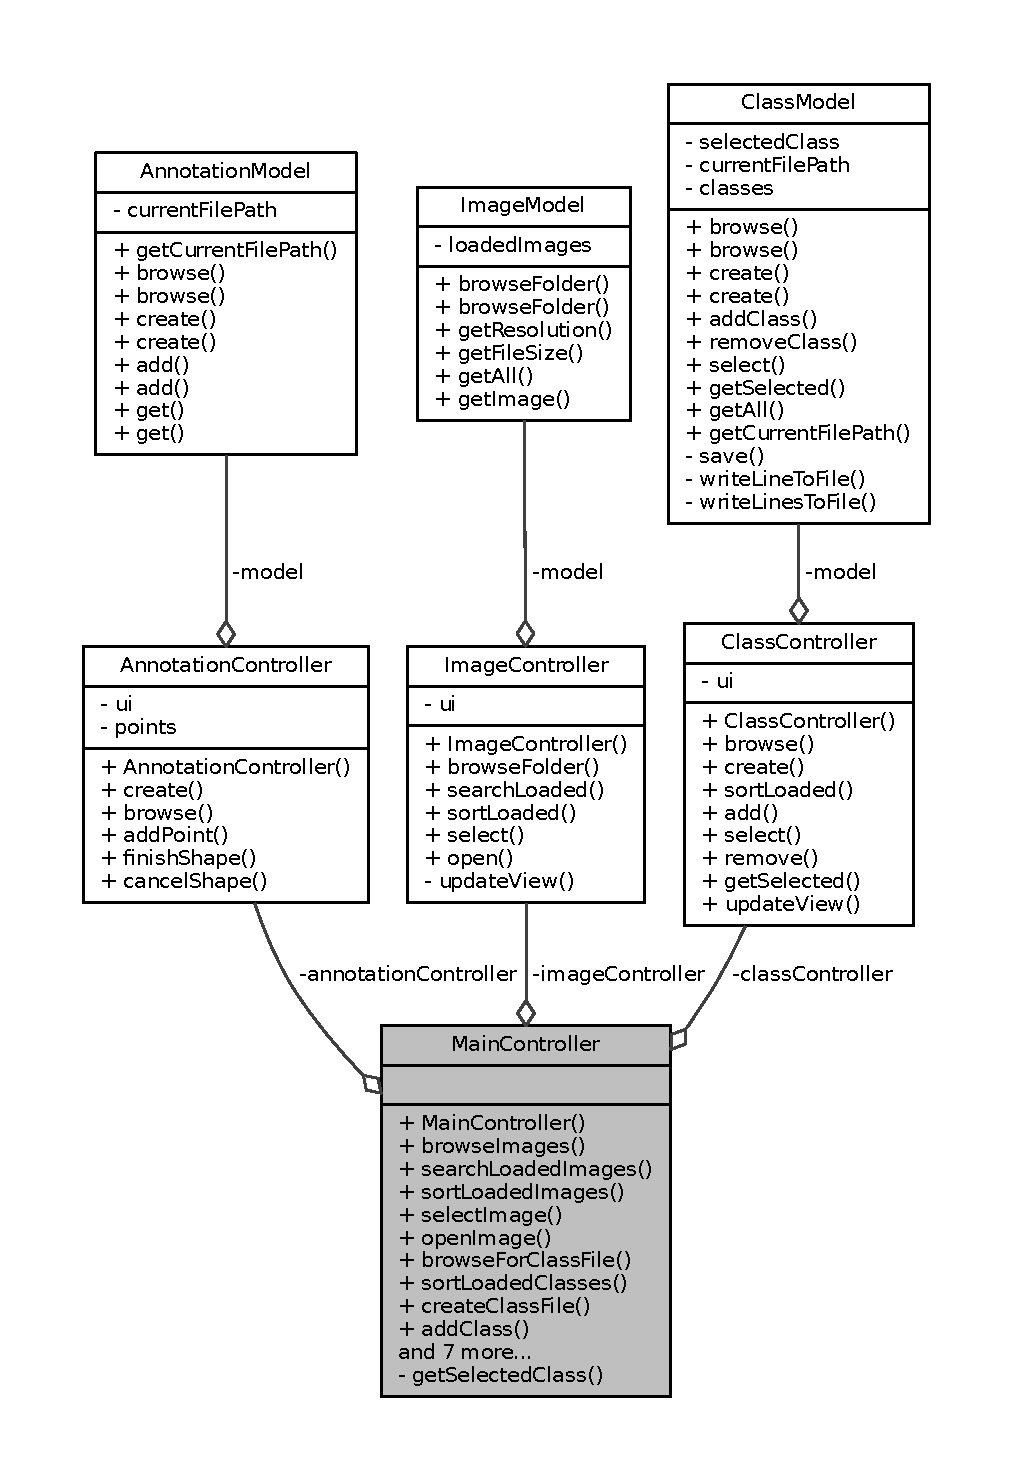
\includegraphics[height=550pt]{classMainController__coll__graph}
\end{center}
\end{figure}
\subsection*{Public Member Functions}
\begin{DoxyCompactItemize}
\item 
\hyperlink{classMainController_a1ec0f2ef4a8efce169354c525afec025}{Main\+Controller} (\hyperlink{classAnnotationController}{Annotation\+Controller} \&, \hyperlink{classClassController}{Class\+Controller} \&, \hyperlink{classImageController}{Image\+Controller} \&)
\begin{DoxyCompactList}\small\item\em Constructs a \hyperlink{classMainController}{Main\+Controller}, taking in references to each type of sub-\/controller. \end{DoxyCompactList}\item 
\mbox{\Hypertarget{classMainController_a9839c3a1b6fac7c4ee47479f86666c2b}\label{classMainController_a9839c3a1b6fac7c4ee47479f86666c2b}} 
void \hyperlink{classMainController_a9839c3a1b6fac7c4ee47479f86666c2b}{browse\+Images} ()
\begin{DoxyCompactList}\small\item\em Delegates the image folder browsing event to the \hyperlink{classImageController}{Image\+Controller}. \end{DoxyCompactList}\item 
\mbox{\Hypertarget{classMainController_a9513dcff8f9540bba40a69b858596961}\label{classMainController_a9513dcff8f9540bba40a69b858596961}} 
void {\bfseries search\+Loaded\+Images} (const Q\+String \&)
\item 
void \hyperlink{classMainController_ad131b9aae76e43061554feed80bb13a2}{sort\+Loaded\+Images} (const Q\+String \&, bool=false)
\begin{DoxyCompactList}\small\item\em Sorts the loaded images and updates the view. \end{DoxyCompactList}\item 
void \hyperlink{classMainController_a528a8b9b2aeee5dd416dc1e57da56693}{select\+Image} (const Q\+String \&)
\begin{DoxyCompactList}\small\item\em \hyperlink{classMainController_a528a8b9b2aeee5dd416dc1e57da56693}{Main\+Controller\+::select\+Image}. \end{DoxyCompactList}\item 
void \hyperlink{classMainController_a44cb414d5932db864383b9cb17c6f0b1}{open\+Image} (const Q\+String \&)
\begin{DoxyCompactList}\small\item\em Gets the image filename from the \hyperlink{classMainView}{Main\+View} and passes request to open image to \hyperlink{classMainController}{Main\+Controller}. \end{DoxyCompactList}\item 
\mbox{\Hypertarget{classMainController_aa717950c16ef5d01ab4edf77a9a27f82}\label{classMainController_aa717950c16ef5d01ab4edf77a9a27f82}} 
void \hyperlink{classMainController_aa717950c16ef5d01ab4edf77a9a27f82}{browse\+For\+Class\+File} ()
\begin{DoxyCompactList}\small\item\em Delegates class folder browsing event to the \hyperlink{classClassController}{Class\+Controller}. \end{DoxyCompactList}\item 
void \hyperlink{classMainController_a21e18cb936861042e1603c029f3c006e}{sort\+Loaded\+Classes} (const Q\+String \&)
\begin{DoxyCompactList}\small\item\em \hyperlink{classMainController_a21e18cb936861042e1603c029f3c006e}{Main\+Controller\+::sort\+Loaded\+Classes} Sorts the loaded classes. \end{DoxyCompactList}\item 
\mbox{\Hypertarget{classMainController_a6cdee58a8c4ed59ab9a05ab5a15456a6}\label{classMainController_a6cdee58a8c4ed59ab9a05ab5a15456a6}} 
void \hyperlink{classMainController_a6cdee58a8c4ed59ab9a05ab5a15456a6}{create\+Class\+File} ()
\begin{DoxyCompactList}\small\item\em Delegates the creation of a class file to the \hyperlink{classClassController}{Class\+Controller}. \end{DoxyCompactList}\item 
void \hyperlink{classMainController_aede8e00b0ad8f75018f6b62e1cb5e301}{add\+Class} (const Q\+String \&)
\begin{DoxyCompactList}\small\item\em Delegates the addition of a new class to the \hyperlink{classClassController}{Class\+Controller}. \end{DoxyCompactList}\item 
void \hyperlink{classMainController_aa2b2e86d0134c9bb413d74efdd926211}{select\+Class} (const Q\+String \&)
\begin{DoxyCompactList}\small\item\em \hyperlink{classMainController_aa2b2e86d0134c9bb413d74efdd926211}{Main\+Controller\+::select\+Class} Selects a class. \end{DoxyCompactList}\item 
void \hyperlink{classMainController_ad639a2fd588d6fe011701a5168184883}{remove\+Class} (const Q\+String \&)
\begin{DoxyCompactList}\small\item\em Delegates the removal of a class to the \hyperlink{classClassController}{Class\+Controller}. \end{DoxyCompactList}\item 
\mbox{\Hypertarget{classMainController_a018730fa763bed9ef77bb7c2fc994bb8}\label{classMainController_a018730fa763bed9ef77bb7c2fc994bb8}} 
void \hyperlink{classMainController_a018730fa763bed9ef77bb7c2fc994bb8}{browse\+For\+Annotation\+File} ()
\begin{DoxyCompactList}\small\item\em \hyperlink{classMainController_a018730fa763bed9ef77bb7c2fc994bb8}{Main\+Controller\+::browse\+For\+Annotation\+File} Browses for an annotation file. \end{DoxyCompactList}\item 
\mbox{\Hypertarget{classMainController_adcab0ecd57994728c1ad67dafc844179}\label{classMainController_adcab0ecd57994728c1ad67dafc844179}} 
void \hyperlink{classMainController_adcab0ecd57994728c1ad67dafc844179}{create\+Annotation\+File} ()
\begin{DoxyCompactList}\small\item\em Delegates the creation of annotation file to the \hyperlink{classAnnotationController}{Annotation\+Controller}. \end{DoxyCompactList}\item 
\mbox{\Hypertarget{classMainController_a6051544c31fbdeb375a88715b8406b52}\label{classMainController_a6051544c31fbdeb375a88715b8406b52}} 
void \hyperlink{classMainController_a6051544c31fbdeb375a88715b8406b52}{save\+Annotations} ()
\begin{DoxyCompactList}\small\item\em \hyperlink{classMainController_a6051544c31fbdeb375a88715b8406b52}{Main\+Controller\+::save\+Annotations} Saves annotations. \end{DoxyCompactList}\item 
void \hyperlink{classMainController_a215cb23587a572993fb00b0c09a393e2}{add\+Point} (Q\+Point)
\begin{DoxyCompactList}\small\item\em \hyperlink{classMainController_a215cb23587a572993fb00b0c09a393e2}{Main\+Controller\+::add\+Point} Adds a point. \end{DoxyCompactList}\item 
\mbox{\Hypertarget{classMainController_afa0ea947f033ff9fac5b798378d03667}\label{classMainController_afa0ea947f033ff9fac5b798378d03667}} 
void \hyperlink{classMainController_afa0ea947f033ff9fac5b798378d03667}{finish\+Shape} ()
\begin{DoxyCompactList}\small\item\em \hyperlink{classMainController_afa0ea947f033ff9fac5b798378d03667}{Main\+Controller\+::finish\+Shape} Finish annotating a shape. \end{DoxyCompactList}\item 
\mbox{\Hypertarget{classMainController_a7855f2a07593bd632e36bed1452386b2}\label{classMainController_a7855f2a07593bd632e36bed1452386b2}} 
void \hyperlink{classMainController_a7855f2a07593bd632e36bed1452386b2}{cancel\+Shape} ()
\begin{DoxyCompactList}\small\item\em \hyperlink{classMainController_a7855f2a07593bd632e36bed1452386b2}{Main\+Controller\+::cancel\+Shape} Cancel annotating a shape. \end{DoxyCompactList}\end{DoxyCompactItemize}
\subsection*{Static Public Member Functions}
\begin{DoxyCompactItemize}
\item 
static void \hyperlink{classMainController_ae4fbe8a429f2181ae8e6c721ea7b113b}{annotation\+Saving\+Thread} (\hyperlink{classMainController}{Main\+Controller} $\ast$)
\begin{DoxyCompactList}\small\item\em \hyperlink{classMainController_ae4fbe8a429f2181ae8e6c721ea7b113b}{Main\+Controller\+::annotation\+Saving\+Thread} Thread which saves annotations every minute. \end{DoxyCompactList}\end{DoxyCompactItemize}
\subsection*{Private Member Functions}
\begin{DoxyCompactItemize}
\item 
Q\+String \hyperlink{classMainController_a1ffca82d85f234d7427385dd28bb2160}{get\+Selected\+Class} ()
\begin{DoxyCompactList}\small\item\em \hyperlink{classMainController_a1ffca82d85f234d7427385dd28bb2160}{Main\+Controller\+::get\+Selected\+Class} Returns the selected class. \end{DoxyCompactList}\end{DoxyCompactItemize}
\subsection*{Private Attributes}
\begin{DoxyCompactItemize}
\item 
\mbox{\Hypertarget{classMainController_af065a8fdd42311f90d96b68f77f2248f}\label{classMainController_af065a8fdd42311f90d96b68f77f2248f}} 
\hyperlink{classAnnotationController}{Annotation\+Controller} {\bfseries annotation\+Controller}
\item 
\mbox{\Hypertarget{classMainController_a5061629143625f07d1131a4ea8d39d73}\label{classMainController_a5061629143625f07d1131a4ea8d39d73}} 
\hyperlink{classClassController}{Class\+Controller} {\bfseries class\+Controller}
\item 
\mbox{\Hypertarget{classMainController_a6553221dd7d26251572bd730fdd9aae5}\label{classMainController_a6553221dd7d26251572bd730fdd9aae5}} 
\hyperlink{classImageController}{Image\+Controller} {\bfseries image\+Controller}
\end{DoxyCompactItemize}


\subsection{Detailed Description}
Processes callbacks from the G\+UI by delegating to the specific sub-\/controllers. Servers as an added layer of separation between the views and controllers to decrease coupling and handles business logic, which spans multiple controllers and models. 

\subsection{Constructor \& Destructor Documentation}
\mbox{\Hypertarget{classMainController_a1ec0f2ef4a8efce169354c525afec025}\label{classMainController_a1ec0f2ef4a8efce169354c525afec025}} 
\index{Main\+Controller@{Main\+Controller}!Main\+Controller@{Main\+Controller}}
\index{Main\+Controller@{Main\+Controller}!Main\+Controller@{Main\+Controller}}
\subsubsection{\texorpdfstring{Main\+Controller()}{MainController()}}
{\footnotesize\ttfamily Main\+Controller\+::\+Main\+Controller (\begin{DoxyParamCaption}\item[{\hyperlink{classAnnotationController}{Annotation\+Controller} \&}]{annotation\+Controller,  }\item[{\hyperlink{classClassController}{Class\+Controller} \&}]{class\+Controller,  }\item[{\hyperlink{classImageController}{Image\+Controller} \&}]{image\+Controller }\end{DoxyParamCaption})}



Constructs a \hyperlink{classMainController}{Main\+Controller}, taking in references to each type of sub-\/controller. 


\begin{DoxyParams}{Parameters}
{\em annotation\+Controller} & \\
\hline
{\em class\+Controller} & \\
\hline
{\em image\+Controller} & \\
\hline
\end{DoxyParams}


\subsection{Member Function Documentation}
\mbox{\Hypertarget{classMainController_aede8e00b0ad8f75018f6b62e1cb5e301}\label{classMainController_aede8e00b0ad8f75018f6b62e1cb5e301}} 
\index{Main\+Controller@{Main\+Controller}!add\+Class@{add\+Class}}
\index{add\+Class@{add\+Class}!Main\+Controller@{Main\+Controller}}
\subsubsection{\texorpdfstring{add\+Class()}{addClass()}}
{\footnotesize\ttfamily void Main\+Controller\+::add\+Class (\begin{DoxyParamCaption}\item[{const Q\+String \&}]{class\+Name }\end{DoxyParamCaption})}



Delegates the addition of a new class to the \hyperlink{classClassController}{Class\+Controller}. 


\begin{DoxyParams}{Parameters}
{\em classname} & Name of the class to add. \\
\hline
\end{DoxyParams}
\mbox{\Hypertarget{classMainController_a215cb23587a572993fb00b0c09a393e2}\label{classMainController_a215cb23587a572993fb00b0c09a393e2}} 
\index{Main\+Controller@{Main\+Controller}!add\+Point@{add\+Point}}
\index{add\+Point@{add\+Point}!Main\+Controller@{Main\+Controller}}
\subsubsection{\texorpdfstring{add\+Point()}{addPoint()}}
{\footnotesize\ttfamily void Main\+Controller\+::add\+Point (\begin{DoxyParamCaption}\item[{Q\+Point}]{point }\end{DoxyParamCaption})}



\hyperlink{classMainController_a215cb23587a572993fb00b0c09a393e2}{Main\+Controller\+::add\+Point} Adds a point. 


\begin{DoxyParams}{Parameters}
{\em point} & \\
\hline
\end{DoxyParams}
\mbox{\Hypertarget{classMainController_ae4fbe8a429f2181ae8e6c721ea7b113b}\label{classMainController_ae4fbe8a429f2181ae8e6c721ea7b113b}} 
\index{Main\+Controller@{Main\+Controller}!annotation\+Saving\+Thread@{annotation\+Saving\+Thread}}
\index{annotation\+Saving\+Thread@{annotation\+Saving\+Thread}!Main\+Controller@{Main\+Controller}}
\subsubsection{\texorpdfstring{annotation\+Saving\+Thread()}{annotationSavingThread()}}
{\footnotesize\ttfamily void Main\+Controller\+::annotation\+Saving\+Thread (\begin{DoxyParamCaption}\item[{\hyperlink{classMainController}{Main\+Controller} $\ast$}]{controller }\end{DoxyParamCaption})\hspace{0.3cm}{\ttfamily [static]}}



\hyperlink{classMainController_ae4fbe8a429f2181ae8e6c721ea7b113b}{Main\+Controller\+::annotation\+Saving\+Thread} Thread which saves annotations every minute. 


\begin{DoxyParams}{Parameters}
{\em controller} & \\
\hline
\end{DoxyParams}
\mbox{\Hypertarget{classMainController_a1ffca82d85f234d7427385dd28bb2160}\label{classMainController_a1ffca82d85f234d7427385dd28bb2160}} 
\index{Main\+Controller@{Main\+Controller}!get\+Selected\+Class@{get\+Selected\+Class}}
\index{get\+Selected\+Class@{get\+Selected\+Class}!Main\+Controller@{Main\+Controller}}
\subsubsection{\texorpdfstring{get\+Selected\+Class()}{getSelectedClass()}}
{\footnotesize\ttfamily Q\+String Main\+Controller\+::get\+Selected\+Class (\begin{DoxyParamCaption}{ }\end{DoxyParamCaption})\hspace{0.3cm}{\ttfamily [private]}}



\hyperlink{classMainController_a1ffca82d85f234d7427385dd28bb2160}{Main\+Controller\+::get\+Selected\+Class} Returns the selected class. 

\begin{DoxyReturn}{Returns}
Q\+String 
\end{DoxyReturn}
\mbox{\Hypertarget{classMainController_a44cb414d5932db864383b9cb17c6f0b1}\label{classMainController_a44cb414d5932db864383b9cb17c6f0b1}} 
\index{Main\+Controller@{Main\+Controller}!open\+Image@{open\+Image}}
\index{open\+Image@{open\+Image}!Main\+Controller@{Main\+Controller}}
\subsubsection{\texorpdfstring{open\+Image()}{openImage()}}
{\footnotesize\ttfamily void Main\+Controller\+::open\+Image (\begin{DoxyParamCaption}\item[{const Q\+String \&}]{file\+Name }\end{DoxyParamCaption})}



Gets the image filename from the \hyperlink{classMainView}{Main\+View} and passes request to open image to \hyperlink{classMainController}{Main\+Controller}. 


\begin{DoxyParams}{Parameters}
{\em filename} & \\
\hline
\end{DoxyParams}
\mbox{\Hypertarget{classMainController_ad639a2fd588d6fe011701a5168184883}\label{classMainController_ad639a2fd588d6fe011701a5168184883}} 
\index{Main\+Controller@{Main\+Controller}!remove\+Class@{remove\+Class}}
\index{remove\+Class@{remove\+Class}!Main\+Controller@{Main\+Controller}}
\subsubsection{\texorpdfstring{remove\+Class()}{removeClass()}}
{\footnotesize\ttfamily void Main\+Controller\+::remove\+Class (\begin{DoxyParamCaption}\item[{const Q\+String \&}]{class\+Name }\end{DoxyParamCaption})}



Delegates the removal of a class to the \hyperlink{classClassController}{Class\+Controller}. 


\begin{DoxyParams}{Parameters}
{\em class\+Name} & Name of the class to remove. \\
\hline
\end{DoxyParams}
\mbox{\Hypertarget{classMainController_aa2b2e86d0134c9bb413d74efdd926211}\label{classMainController_aa2b2e86d0134c9bb413d74efdd926211}} 
\index{Main\+Controller@{Main\+Controller}!select\+Class@{select\+Class}}
\index{select\+Class@{select\+Class}!Main\+Controller@{Main\+Controller}}
\subsubsection{\texorpdfstring{select\+Class()}{selectClass()}}
{\footnotesize\ttfamily void Main\+Controller\+::select\+Class (\begin{DoxyParamCaption}\item[{const Q\+String \&}]{class\+Name }\end{DoxyParamCaption})}



\hyperlink{classMainController_aa2b2e86d0134c9bb413d74efdd926211}{Main\+Controller\+::select\+Class} Selects a class. 


\begin{DoxyParams}{Parameters}
{\em class\+Name} & \\
\hline
\end{DoxyParams}
\mbox{\Hypertarget{classMainController_a528a8b9b2aeee5dd416dc1e57da56693}\label{classMainController_a528a8b9b2aeee5dd416dc1e57da56693}} 
\index{Main\+Controller@{Main\+Controller}!select\+Image@{select\+Image}}
\index{select\+Image@{select\+Image}!Main\+Controller@{Main\+Controller}}
\subsubsection{\texorpdfstring{select\+Image()}{selectImage()}}
{\footnotesize\ttfamily void Main\+Controller\+::select\+Image (\begin{DoxyParamCaption}\item[{const Q\+String \&}]{file\+Name }\end{DoxyParamCaption})}



\hyperlink{classMainController_a528a8b9b2aeee5dd416dc1e57da56693}{Main\+Controller\+::select\+Image}. 


\begin{DoxyParams}{Parameters}
{\em file\+Name} & \\
\hline
\end{DoxyParams}
\mbox{\Hypertarget{classMainController_a21e18cb936861042e1603c029f3c006e}\label{classMainController_a21e18cb936861042e1603c029f3c006e}} 
\index{Main\+Controller@{Main\+Controller}!sort\+Loaded\+Classes@{sort\+Loaded\+Classes}}
\index{sort\+Loaded\+Classes@{sort\+Loaded\+Classes}!Main\+Controller@{Main\+Controller}}
\subsubsection{\texorpdfstring{sort\+Loaded\+Classes()}{sortLoadedClasses()}}
{\footnotesize\ttfamily void Main\+Controller\+::sort\+Loaded\+Classes (\begin{DoxyParamCaption}\item[{const Q\+String \&}]{sort\+Option }\end{DoxyParamCaption})}



\hyperlink{classMainController_a21e18cb936861042e1603c029f3c006e}{Main\+Controller\+::sort\+Loaded\+Classes} Sorts the loaded classes. 


\begin{DoxyParams}{Parameters}
{\em sort\+Option} & \\
\hline
\end{DoxyParams}
\mbox{\Hypertarget{classMainController_ad131b9aae76e43061554feed80bb13a2}\label{classMainController_ad131b9aae76e43061554feed80bb13a2}} 
\index{Main\+Controller@{Main\+Controller}!sort\+Loaded\+Images@{sort\+Loaded\+Images}}
\index{sort\+Loaded\+Images@{sort\+Loaded\+Images}!Main\+Controller@{Main\+Controller}}
\subsubsection{\texorpdfstring{sort\+Loaded\+Images()}{sortLoadedImages()}}
{\footnotesize\ttfamily void Main\+Controller\+::sort\+Loaded\+Images (\begin{DoxyParamCaption}\item[{const Q\+String \&}]{sort\+Option,  }\item[{bool}]{srch = {\ttfamily false} }\end{DoxyParamCaption})}



Sorts the loaded images and updates the view. 


\begin{DoxyParams}{Parameters}
{\em sort\+Option} & \\
\hline
{\em srch} & \\
\hline
\end{DoxyParams}


The documentation for this class was generated from the following files\+:\begin{DoxyCompactItemize}
\item 
include/Main\+Controller.\+h\item 
src/Main\+Controller.\+cpp\end{DoxyCompactItemize}

\hypertarget{classMainView}{}\section{Main\+View Class Reference}
\label{classMainView}\index{Main\+View@{Main\+View}}


Inheritance diagram for Main\+View\+:\nopagebreak
\begin{figure}[H]
\begin{center}
\leavevmode
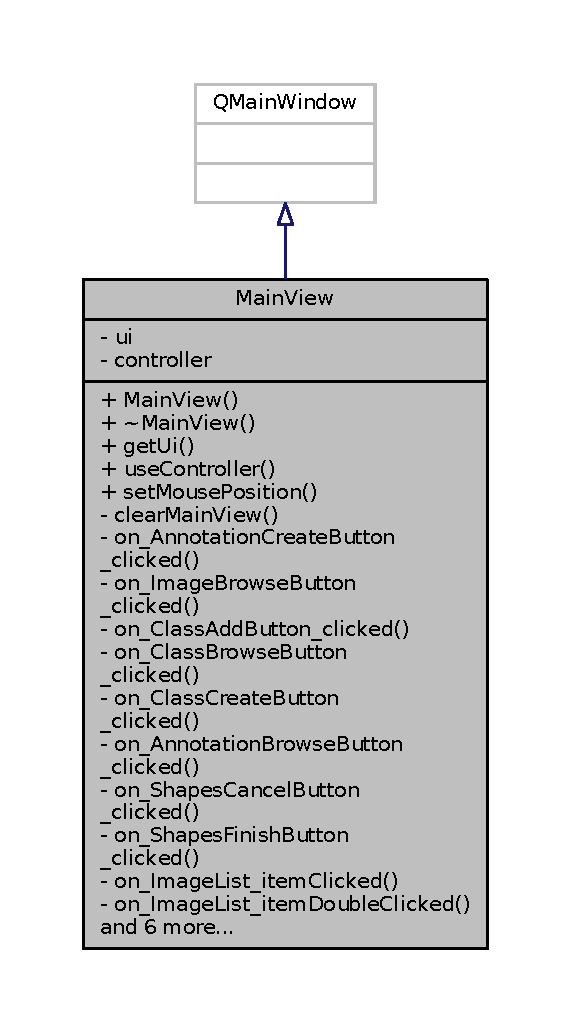
\includegraphics[width=255pt]{classMainView__inherit__graph}
\end{center}
\end{figure}


Collaboration diagram for Main\+View\+:
\nopagebreak
\begin{figure}[H]
\begin{center}
\leavevmode
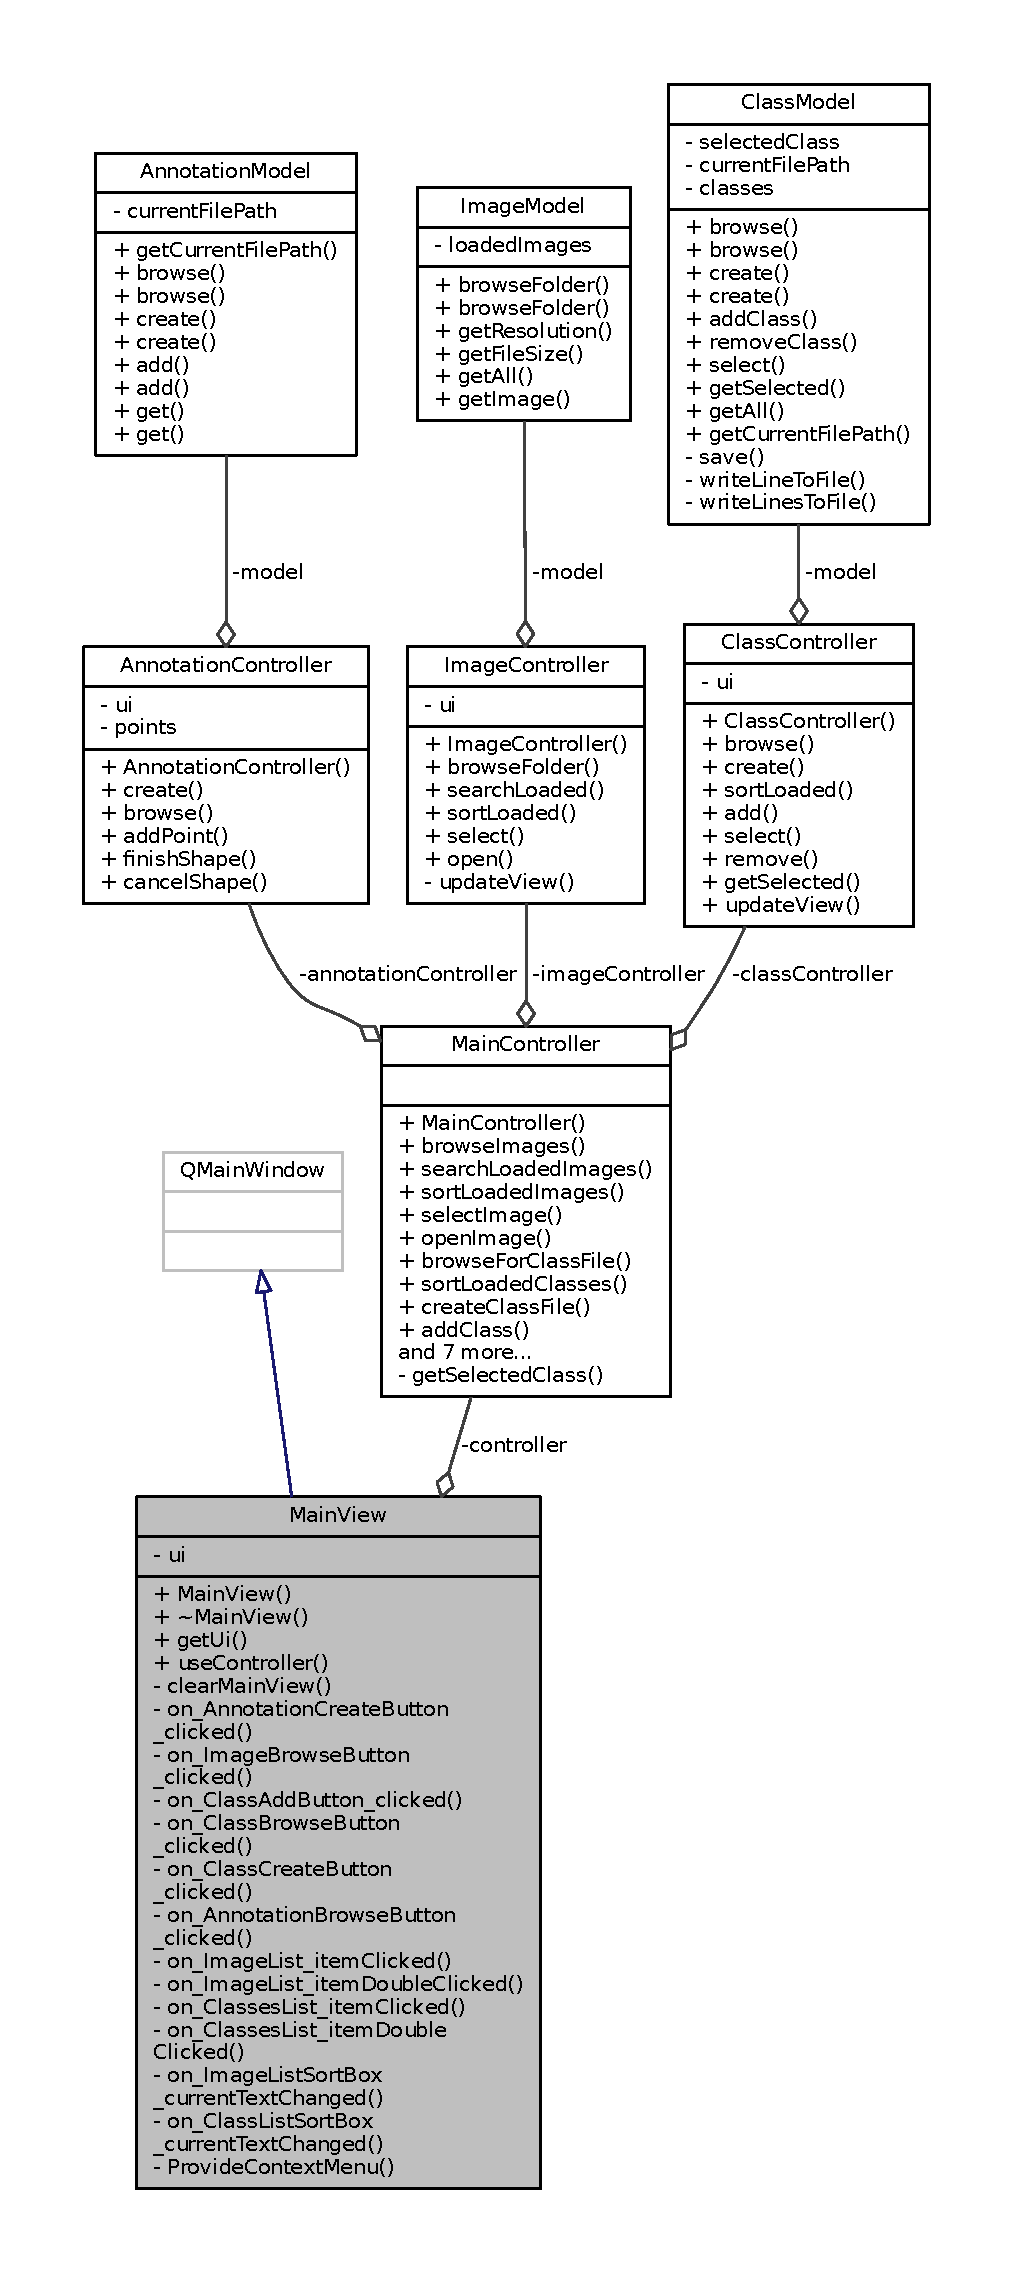
\includegraphics[height=550pt]{classMainView__coll__graph}
\end{center}
\end{figure}
\subsection*{Public Member Functions}
\begin{DoxyCompactItemize}
\item 
\hyperlink{classMainView_a3e82d0020daca697d56361c68556d445}{Main\+View} (Q\+Widget $\ast$parent=nullptr)
\begin{DoxyCompactList}\small\item\em Creates a new internal Ui\+::\+Main\+View object and sets up the G\+UI. \end{DoxyCompactList}\item 
\mbox{\Hypertarget{classMainView_a8c9f70ed683307067d3bc7cbe131d233}\label{classMainView_a8c9f70ed683307067d3bc7cbe131d233}} 
\hyperlink{classMainView_a8c9f70ed683307067d3bc7cbe131d233}{$\sim$\+Main\+View} ()
\begin{DoxyCompactList}\small\item\em Destructs the internal Ui\+::\+Main\+View object. \end{DoxyCompactList}\item 
\mbox{\Hypertarget{classMainView_aa80a128b57958154012b0e4339f479d5}\label{classMainView_aa80a128b57958154012b0e4339f479d5}} 
Ui\+::\+Main\+View \hyperlink{classMainView_aa80a128b57958154012b0e4339f479d5}{get\+Ui} ()
\begin{DoxyCompactList}\small\item\em Returns a pointer to the internal Ui\+::\+Main\+View object, which is used for processing callbacks. \end{DoxyCompactList}\item 
void \hyperlink{classMainView_a077240bb5f37693cd4764914d69b98eb}{use\+Controller} (\hyperlink{classMainController}{Main\+Controller} $\ast$)
\begin{DoxyCompactList}\small\item\em Passes a \hyperlink{classMainController}{Main\+Controller} pointer to the \hyperlink{classMainView}{Main\+View}, which it uses to process callbacks. \end{DoxyCompactList}\end{DoxyCompactItemize}
\subsection*{Private Slots}
\begin{DoxyCompactItemize}
\item 
\mbox{\Hypertarget{classMainView_af0436aa7323ec0580616b33adc219784}\label{classMainView_af0436aa7323ec0580616b33adc219784}} 
void \hyperlink{classMainView_af0436aa7323ec0580616b33adc219784}{on\+\_\+\+Annotation\+Create\+Button\+\_\+clicked} ()
\begin{DoxyCompactList}\small\item\em Callback function, which is triggered by user clicking on create annotation file button. \end{DoxyCompactList}\item 
\mbox{\Hypertarget{classMainView_a8e170aa23a65f1c7f3ed3a7c08a99101}\label{classMainView_a8e170aa23a65f1c7f3ed3a7c08a99101}} 
void \hyperlink{classMainView_a8e170aa23a65f1c7f3ed3a7c08a99101}{on\+\_\+\+Image\+Browse\+Button\+\_\+clicked} ()
\begin{DoxyCompactList}\small\item\em Callback function, which is triggered by the user clicking the \char`\"{}\+Browse\char`\"{} button in the image panel. \end{DoxyCompactList}\item 
\mbox{\Hypertarget{classMainView_aaa6cd08b912bcc873f9a7c04258f98bb}\label{classMainView_aaa6cd08b912bcc873f9a7c04258f98bb}} 
void {\bfseries on\+\_\+\+Class\+Add\+Button\+\_\+clicked} ()
\item 
\mbox{\Hypertarget{classMainView_a67267813d7c408d32be5e6fef2251a6f}\label{classMainView_a67267813d7c408d32be5e6fef2251a6f}} 
void {\bfseries on\+\_\+\+Class\+Browse\+Button\+\_\+clicked} ()
\item 
\mbox{\Hypertarget{classMainView_a3edf1fc4556c571b3d2130db22da504e}\label{classMainView_a3edf1fc4556c571b3d2130db22da504e}} 
void {\bfseries on\+\_\+\+Class\+Create\+Button\+\_\+clicked} ()
\item 
\mbox{\Hypertarget{classMainView_a4995ea260acd3abf8ac31f148f2415ca}\label{classMainView_a4995ea260acd3abf8ac31f148f2415ca}} 
void {\bfseries on\+\_\+\+Annotation\+Browse\+Button\+\_\+clicked} ()
\item 
\mbox{\Hypertarget{classMainView_a21afbf21cbe8fc3e444d57cd575e69b0}\label{classMainView_a21afbf21cbe8fc3e444d57cd575e69b0}} 
void {\bfseries on\+\_\+\+Image\+List\+\_\+item\+Clicked} (Q\+List\+Widget\+Item $\ast$)
\item 
void \hyperlink{classMainView_ae0af943bbf0d0806261bb8aa5444eb5b}{on\+\_\+\+Image\+List\+\_\+item\+Double\+Clicked} (Q\+List\+Widget\+Item $\ast$)
\begin{DoxyCompactList}\small\item\em Callback function, which is triggered by user double clicking on the image file name in the image pannel. \end{DoxyCompactList}\item 
\mbox{\Hypertarget{classMainView_a2970c289fed50a4d86051135af81ba61}\label{classMainView_a2970c289fed50a4d86051135af81ba61}} 
void {\bfseries on\+\_\+\+Classes\+List\+\_\+item\+Clicked} (Q\+List\+Widget\+Item $\ast$)
\item 
\mbox{\Hypertarget{classMainView_a53645de6ba66e27080df09fc7cbbf3d6}\label{classMainView_a53645de6ba66e27080df09fc7cbbf3d6}} 
void {\bfseries on\+\_\+\+Classes\+List\+\_\+item\+Double\+Clicked} (Q\+List\+Widget\+Item $\ast$)
\item 
\mbox{\Hypertarget{classMainView_ab2b972e9dd92f3f3be8a7b4ac9380698}\label{classMainView_ab2b972e9dd92f3f3be8a7b4ac9380698}} 
void {\bfseries on\+\_\+\+Image\+List\+Sort\+Box\+\_\+current\+Text\+Changed} (const Q\+String \&)
\item 
\mbox{\Hypertarget{classMainView_afb94b7f4f66f2c7f0bc841f9e95b4519}\label{classMainView_afb94b7f4f66f2c7f0bc841f9e95b4519}} 
void {\bfseries on\+\_\+\+Class\+List\+Sort\+Box\+\_\+current\+Text\+Changed} (const Q\+String \&)
\item 
void \hyperlink{classMainView_aa9d5f1300bd6b2524f611873d68c938b}{Provide\+Context\+Menu} (const Q\+Point \&)
\begin{DoxyCompactList}\small\item\em Creates a context menu on right-\/click of the classes pane. \end{DoxyCompactList}\end{DoxyCompactItemize}
\subsection*{Private Member Functions}
\begin{DoxyCompactItemize}
\item 
\mbox{\Hypertarget{classMainView_a38e251a0a33b91a95157b24b105e75fb}\label{classMainView_a38e251a0a33b91a95157b24b105e75fb}} 
void {\bfseries clear\+Main\+View} ()
\end{DoxyCompactItemize}
\subsection*{Private Attributes}
\begin{DoxyCompactItemize}
\item 
\mbox{\Hypertarget{classMainView_ae0f57d2bd69b0609aee18888c8467bb5}\label{classMainView_ae0f57d2bd69b0609aee18888c8467bb5}} 
Ui\+::\+Main\+View $\ast$ {\bfseries ui}
\item 
\mbox{\Hypertarget{classMainView_afd7249923bf85f7cdb24c6807f55400d}\label{classMainView_afd7249923bf85f7cdb24c6807f55400d}} 
\hyperlink{classMainController}{Main\+Controller} $\ast$ {\bfseries controller}
\end{DoxyCompactItemize}


\subsection{Constructor \& Destructor Documentation}
\mbox{\Hypertarget{classMainView_a3e82d0020daca697d56361c68556d445}\label{classMainView_a3e82d0020daca697d56361c68556d445}} 
\index{Main\+View@{Main\+View}!Main\+View@{Main\+View}}
\index{Main\+View@{Main\+View}!Main\+View@{Main\+View}}
\subsubsection{\texorpdfstring{Main\+View()}{MainView()}}
{\footnotesize\ttfamily Main\+View\+::\+Main\+View (\begin{DoxyParamCaption}\item[{Q\+Widget $\ast$}]{parent = {\ttfamily nullptr} }\end{DoxyParamCaption})}



Creates a new internal Ui\+::\+Main\+View object and sets up the G\+UI. 


\begin{DoxyParams}{Parameters}
{\em parent} & \\
\hline
\end{DoxyParams}


\subsection{Member Function Documentation}
\mbox{\Hypertarget{classMainView_ae0af943bbf0d0806261bb8aa5444eb5b}\label{classMainView_ae0af943bbf0d0806261bb8aa5444eb5b}} 
\index{Main\+View@{Main\+View}!on\+\_\+\+Image\+List\+\_\+item\+Double\+Clicked@{on\+\_\+\+Image\+List\+\_\+item\+Double\+Clicked}}
\index{on\+\_\+\+Image\+List\+\_\+item\+Double\+Clicked@{on\+\_\+\+Image\+List\+\_\+item\+Double\+Clicked}!Main\+View@{Main\+View}}
\subsubsection{\texorpdfstring{on\+\_\+\+Image\+List\+\_\+item\+Double\+Clicked}{on\_ImageList\_itemDoubleClicked}}
{\footnotesize\ttfamily void Main\+View\+::on\+\_\+\+Image\+List\+\_\+item\+Double\+Clicked (\begin{DoxyParamCaption}\item[{Q\+List\+Widget\+Item $\ast$}]{file\+Name }\end{DoxyParamCaption})\hspace{0.3cm}{\ttfamily [private]}, {\ttfamily [slot]}}



Callback function, which is triggered by user double clicking on the image file name in the image pannel. 

Then passes request to open image to \hyperlink{classMainController}{Main\+Controller}.


\begin{DoxyParams}{Parameters}
{\em filename} & \\
\hline
\end{DoxyParams}
\mbox{\Hypertarget{classMainView_aa9d5f1300bd6b2524f611873d68c938b}\label{classMainView_aa9d5f1300bd6b2524f611873d68c938b}} 
\index{Main\+View@{Main\+View}!Provide\+Context\+Menu@{Provide\+Context\+Menu}}
\index{Provide\+Context\+Menu@{Provide\+Context\+Menu}!Main\+View@{Main\+View}}
\subsubsection{\texorpdfstring{Provide\+Context\+Menu}{ProvideContextMenu}}
{\footnotesize\ttfamily void Main\+View\+::\+Provide\+Context\+Menu (\begin{DoxyParamCaption}\item[{const Q\+Point \&}]{position }\end{DoxyParamCaption})\hspace{0.3cm}{\ttfamily [private]}, {\ttfamily [slot]}}



Creates a context menu on right-\/click of the classes pane. 


\begin{DoxyParams}{Parameters}
{\em pos} & Position of the cursor. \\
\hline
\end{DoxyParams}
\mbox{\Hypertarget{classMainView_a077240bb5f37693cd4764914d69b98eb}\label{classMainView_a077240bb5f37693cd4764914d69b98eb}} 
\index{Main\+View@{Main\+View}!use\+Controller@{use\+Controller}}
\index{use\+Controller@{use\+Controller}!Main\+View@{Main\+View}}
\subsubsection{\texorpdfstring{use\+Controller()}{useController()}}
{\footnotesize\ttfamily void Main\+View\+::use\+Controller (\begin{DoxyParamCaption}\item[{\hyperlink{classMainController}{Main\+Controller} $\ast$}]{controller }\end{DoxyParamCaption})}



Passes a \hyperlink{classMainController}{Main\+Controller} pointer to the \hyperlink{classMainView}{Main\+View}, which it uses to process callbacks. 


\begin{DoxyParams}{Parameters}
{\em controller} & \\
\hline
\end{DoxyParams}


The documentation for this class was generated from the following files\+:\begin{DoxyCompactItemize}
\item 
include/Main\+View.\+h\item 
src/Main\+View.\+cpp\end{DoxyCompactItemize}

\hypertarget{structLinkedList_1_1Node}{}\section{Linked\+List$<$ T $>$\+:\+:Node Struct Reference}
\label{structLinkedList_1_1Node}\index{Linked\+List$<$ T $>$\+::\+Node@{Linked\+List$<$ T $>$\+::\+Node}}


Collaboration diagram for Linked\+List$<$ T $>$\+:\+:Node\+:\nopagebreak
\begin{figure}[H]
\begin{center}
\leavevmode
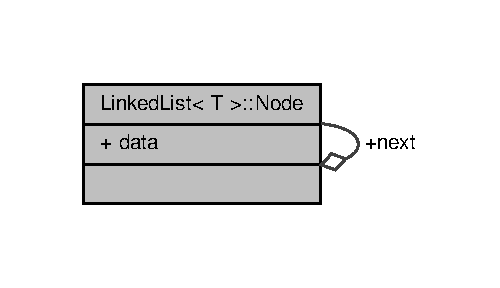
\includegraphics[width=240pt]{structLinkedList_1_1Node__coll__graph}
\end{center}
\end{figure}
\subsection*{Public Attributes}
\begin{DoxyCompactItemize}
\item 
\mbox{\Hypertarget{structLinkedList_1_1Node_ad2de6fe830fed52d6782ff2caacc51ac}\label{structLinkedList_1_1Node_ad2de6fe830fed52d6782ff2caacc51ac}} 
T {\bfseries data}
\item 
\mbox{\Hypertarget{structLinkedList_1_1Node_aaf5f5d6645d0854e3ed2493bbea57f78}\label{structLinkedList_1_1Node_aaf5f5d6645d0854e3ed2493bbea57f78}} 
\hyperlink{structLinkedList_1_1Node}{Node} $\ast$ {\bfseries next}
\end{DoxyCompactItemize}


The documentation for this struct was generated from the following file\+:\begin{DoxyCompactItemize}
\item 
include/Linked\+List.\+h\end{DoxyCompactItemize}

\hypertarget{classOperationCanceled}{}\section{Operation\+Canceled Class Reference}
\label{classOperationCanceled}\index{Operation\+Canceled@{Operation\+Canceled}}


Inheritance diagram for Operation\+Canceled\+:\nopagebreak
\begin{figure}[H]
\begin{center}
\leavevmode
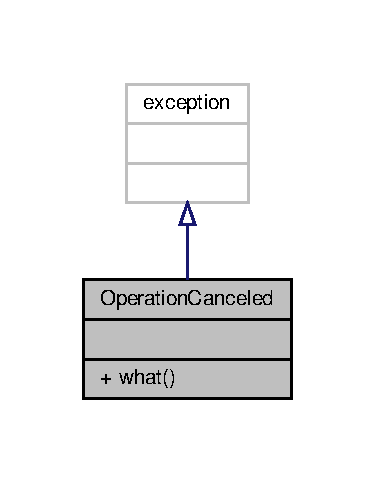
\includegraphics[width=180pt]{classOperationCanceled__inherit__graph}
\end{center}
\end{figure}


Collaboration diagram for Operation\+Canceled\+:\nopagebreak
\begin{figure}[H]
\begin{center}
\leavevmode
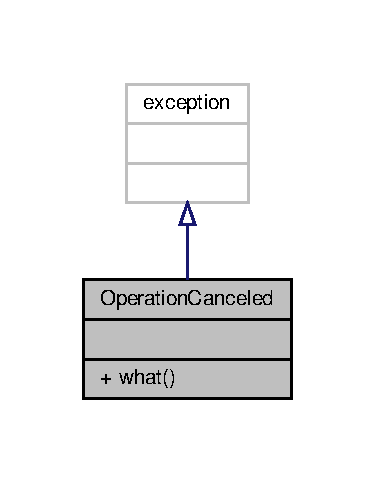
\includegraphics[width=180pt]{classOperationCanceled__coll__graph}
\end{center}
\end{figure}
\subsection*{Public Member Functions}
\begin{DoxyCompactItemize}
\item 
\mbox{\Hypertarget{classOperationCanceled_ae544f829d25de3cd4221c9912e21d7a1}\label{classOperationCanceled_ae544f829d25de3cd4221c9912e21d7a1}} 
const char $\ast$ {\bfseries what} () const  throw ()
\end{DoxyCompactItemize}


The documentation for this class was generated from the following file\+:\begin{DoxyCompactItemize}
\item 
include/exceptions.\+h\end{DoxyCompactItemize}

\hypertarget{classValueNotFoundError}{}\section{Value\+Not\+Found\+Error Class Reference}
\label{classValueNotFoundError}\index{Value\+Not\+Found\+Error@{Value\+Not\+Found\+Error}}


Inheritance diagram for Value\+Not\+Found\+Error\+:\nopagebreak
\begin{figure}[H]
\begin{center}
\leavevmode
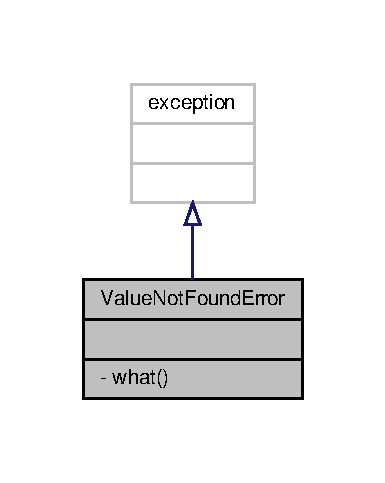
\includegraphics[width=185pt]{classValueNotFoundError__inherit__graph}
\end{center}
\end{figure}


Collaboration diagram for Value\+Not\+Found\+Error\+:\nopagebreak
\begin{figure}[H]
\begin{center}
\leavevmode
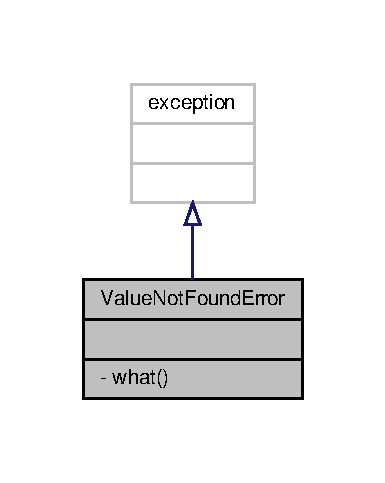
\includegraphics[width=185pt]{classValueNotFoundError__coll__graph}
\end{center}
\end{figure}
\subsection*{Private Member Functions}
\begin{DoxyCompactItemize}
\item 
\mbox{\Hypertarget{classValueNotFoundError_a46595dbe7471a2b20ee246bceec01487}\label{classValueNotFoundError_a46595dbe7471a2b20ee246bceec01487}} 
const char $\ast$ {\bfseries what} () const  throw ()
\end{DoxyCompactItemize}


The documentation for this class was generated from the following file\+:\begin{DoxyCompactItemize}
\item 
include/exceptions.\+h\end{DoxyCompactItemize}

%--- End generated contents ---

% Index
\backmatter
\newpage
\phantomsection
\clearemptydoublepage
\addcontentsline{toc}{chapter}{Index}
\printindex

\end{document}
